% $Id: BASENAME.tex 24073 2019-04-17 23:28:25Z anderson $
% ---------------------------------------------------------
%     DO NOT EDIT THIS FILE - ALL CHANGES WILL BE LOST    
%
% This is the top-level file for PDG review databases. It
% is automatically generated and updated based on the PDG
% database and using the latest PDG LaTeX templates.
%
% Please edit the file databases-main.tex to update your
% review.
% ---------------------------------------------------------

\documentclass{pdg}

% Data extracted from the PDG database
%
% NOTE: - \ischaptertrue or \ischapterfalse determine whether chapter is numbered or not
%       - \sectiontitle set to non-blank value indicates a subreview (or subsubreview)
%       - \subsectiontitle set to non-blank value indicates a subsubreview
%
\reviewtitle{Online Particle Physics Information}
\reviewauthor{A. Holtkamp (CERN) and M. Moskovic (CERN)}
\reviewlabel{databases}
\ischapterfalse

% Include review (and if applicable, subreview) preamble files
% $Id: BASENAME-preamble.tex 23033 2018-09-28 23:38:29Z beringer $
% File for including review-specific LaTeX commands that must appear in the preamble.
% The primary use of this file is to include any additional LaTeX packages.


% compatibility for pandoc generated LaTeX
\newcommand{\tightlist}{}
\let\oldurl\url
\renewcommand{\url}[1]{\begin{center}\indent\oldurl{#1}\end{center}}


% In draft mode, add index
\ifdefined\isdraft
\usepackage{makeidx}
\makeindex
\fi

\ifdefined\isbooklet
\externalcitedocument{databases-full}
\externaldocument{databases-full}
\fi

% Start document, add top-level review title (and possibly section) for subreviews
\begin{document}

% Include -main or -booklet file, depending on what we're making
\ifdefined\isbooklet
\fontsize{8pt}{9pt}\selectfont
\input{databases-booklet}
\else
\begin{bibunit}
% $Id: BASENAME-main.tex 23686 2019-02-20 20:00:48Z beringer $
% Main file for PDG review databases
%
% This file is included by the top-level file databases.tex and is where the
% text of your review should be included. If desired, you may split your review into multiple
% files that are included from this file using \input.
%
% Do NOT modify the top-level file databases.tex - it is generated from
% the PDG database and all manual changes WILL BE LOST!


% Review title
% ------------
% Please use \pdgtitle (rather than e.g. \chapter) to put the title of your review.
%
% To put the review title extracted from the PDG database, use \pdgtitle (no arguments).
% To override the default review title, you can use \pdgtitle[Some different title].
% In the latter case, please ask your overseer to update the review title in the database
\pdgtitle


% Table of contents
% -----------------
% If you want to include a table of contents at the start of your review,
% uncomment the line below. This should only be done for relatively long
% reviews.
%\tableofcontents


% Author information for this review
% ----------------------------------
% Please use one of the following forms:
%   \written{month year}
%   \revised{month year}
%   \customauthor{...}
% The first two, \written and \revised take the month and year when the review
% was written or revised as their only argument. The author list is generated
% from the PDG database. This is the preferred way of including author information.
% Only if really needed, you may use the third from, \customauthor, where you can
% specify the full text of the paragraph giving the review author information.
\revised{August 2019}


% Sectioning
% ----------
% This review is a regular review, please use \section for your top-level sectioning.
% For example:
%\section{Your first section title}


% Text of your review
% -------------------
% Please see the instructions at https://pdgdoc.lbl.gov/Pdg/ReviewTool on how to
% include figures, tables, and references. By default we include file examples.tex,
% which provides instructions and examples of how to include figures, tables, how
% to align equations, and more. It also produces an appendix showing all the standard
% PDG symbols and what they produce.
%
% To remove the examples from your review, comment out the following line when you
% start writing your review.
%% This is the LaTeX source file for the instructions on typesetting PDG
% reviews. It is included with your review source files so you can include
% these instructions into your own review and see some examples.
%
% These same instructions are also provided as a standalone PDF file
% in instructions.pdf.
%
% ---------- Special definitions for PDG review instructions ----------
% The following redefinitions ensure that the example documentation is
% inserted at the correct section level in user reviews:
\let\Isection\section
\let\Isubsection\subsection

\lstdefinestyle{tex}{
	language={[LaTeX]TeX},
	%alsoletter={\\,*,\&},
	basicstyle=\footnotesize\ttfamily,
	texcsstyle=*\ttfamily\color{blue!50!gray},
	keywordstyle=\ttfamily\color{blue!60!gray},
	stringstyle=\ttfamily\color{red!60!gray},
	commentstyle=\ttfamily\color{black!50}, 
	moredelim=**[s][\ttfamily\color{red!60!gray}]{<}{>},
	mathescape,
	%columns=fixed,
    	showtabs=false,
   	keepspaces,
	upquote=true, 
	showstringspaces=false,
	tabsize=4,
	morekeywords={bookcr,bookletcr,webcr,bookalign,bookletalign,webalign,includegraphics,
	setfootnotestyle,captionsetup,rotatebox,multicolumn, multirow, multispan, makecell, iswebbook,balancedlastpagefalse,blankendpagetrue,crossref,tag,xspace},
	breakatwhitespace,
	%literate={>}{}{0},
}
\lstset{style=tex}
\lstnewenvironment{verbtex}{}{}
\newcommand{\invt}[1]{\lstinline!#1!}

%TOC depth
\setcounter{tocdepth}{4}
\setlength{\cftsecnumwidth}{6em} 
\setlength{\cftsubsecnumwidth}{6em} 
\tableofcontents
\setlength{\parskip}{5pt} 
% ---------- End of special definitions for PDG review instructions ----------


\Isection{Typesetting PDG reviews}
These instructions contain documentation and examples for typesetting PDG reviews using the PDG \LaTeX \ class.

They are initially included in the template source files for your own review as an example.
Once you begin writing your review, you should comment out the \lstinline!% This is the LaTeX source file for the instructions on typesetting PDG
% reviews. It is included with your review source files so you can include
% these instructions into your own review and see some examples.
%
% These same instructions are also provided as a standalone PDF file
% in instructions.pdf.
%
% ---------- Special definitions for PDG review instructions ----------
% The following redefinitions ensure that the example documentation is
% inserted at the correct section level in user reviews:
\let\Isection\section
\let\Isubsection\subsection

\lstdefinestyle{tex}{
	language={[LaTeX]TeX},
	%alsoletter={\\,*,\&},
	basicstyle=\footnotesize\ttfamily,
	texcsstyle=*\ttfamily\color{blue!50!gray},
	keywordstyle=\ttfamily\color{blue!60!gray},
	stringstyle=\ttfamily\color{red!60!gray},
	commentstyle=\ttfamily\color{black!50}, 
	moredelim=**[s][\ttfamily\color{red!60!gray}]{<}{>},
	mathescape,
	%columns=fixed,
    	showtabs=false,
   	keepspaces,
	upquote=true, 
	showstringspaces=false,
	tabsize=4,
	morekeywords={bookcr,bookletcr,webcr,bookalign,bookletalign,webalign,includegraphics,
	setfootnotestyle,captionsetup,rotatebox,multicolumn, multirow, multispan, makecell, iswebbook,balancedlastpagefalse,blankendpagetrue,crossref,tag,xspace},
	breakatwhitespace,
	%literate={>}{}{0},
}
\lstset{style=tex}
\lstnewenvironment{verbtex}{}{}
\newcommand{\invt}[1]{\lstinline!#1!}

%TOC depth
\setcounter{tocdepth}{4}
\setlength{\cftsecnumwidth}{6em} 
\setlength{\cftsubsecnumwidth}{6em} 
\tableofcontents
\setlength{\parskip}{5pt} 
% ---------- End of special definitions for PDG review instructions ----------


\Isection{Typesetting PDG reviews}
These instructions contain documentation and examples for typesetting PDG reviews using the PDG \LaTeX \ class.

They are initially included in the template source files for your own review as an example.
Once you begin writing your review, you should comment out the \lstinline!\input{examples.tex}! line that includes these instructions in the main source file of your review, \invt{databases-main.tex}.

This documentation focuses mostly on the specialized functionality of the PDG \LaTeX \ class: %There are many resources that provide more general guidance for typesetting in \LaTeX.
For further support, or any \LaTeX-related questions, we invite authors to contact
\vspace{-0.2cm}
\begin{center}
\scalebox{1.5}{
	\invt{latexsupport@pdg.lbl.gov}
}
\end{center}

\Isubsection{File structure}
The source files for a PDG review are kept in separate directories within a SVN repository. 
Some files in each directory are auto-generated, while others are designed to be edited by review authors. 
\textbf{Do not edit auto-generated files, as any edits to these files will be overwritten periodically.}

Each review is assigned a unique name ("basename") that is used to label the relevant review files and will be referred to as \invt{BASENAME} in the following. For example, the QCD review is assigned basename \invt{qcd}. Therefore \invt{BASENAME-main.tex} in this documentation refers to file \invt{qcd-main.tex} for the QCD review.

Your review is assigned basename \invt{databases}.

The basename is further used to label cross-references to the review (see Sec.~\ref{sec:labels}) and specialized citations (see Sec.~\ref{sec:cites}). 
The file structure of a typical review is as follows:
\begin{itemize}
\item \invt{BASENAME-main.tex} --- contains the text of your review. 
\item \invt{BASENAME-booklet.tex} --- contains the text of the booklet version of your review (if there is one)
\item \invt{BASENAME-preamble.tex} --- contains review-specific definitions or inclusion of packages, that need to go into the document's preamble
\item \invt{BASENAME.bib} --- BibTeX bibliography entries (see Sec~\ref{sec:cites})
\item \invt{/figures} --- directory containing all figures
\item Auxiliary files (\invt{.aux}, \invt{.out}, \invt{.log}) --- these are generated by the \LaTeX compiler
\item Other \invt{.tex} files --- may be added and included in \invt{BASENAME-main.tex} or \invt{BASENAME-booklet.tex} with the \lstinline{\input} command.
\item \textbf{[auto-generated]} \invt{BASENAME.tex} --- compilation file for the review
\item \textbf{[auto-generated]} \invt{Makefile} --- Makefile to compile the review automatically (see Sec.~\ref{sec:make})
\item \textbf{[auto-generated]} \invt{pdg.cls} --- PDG \LaTeX \ class file
\item \textbf{[auto-generated]} \invt{pdg.bst} --- BibTeX PDG style file
\item \textbf{[auto-generated]} \invt{pdg-xr-hyper.sty} --- helper BibTeX style file
\item \textbf{[auto-generated]} \invt{pdgdefs.tex} --- PDG standard symbols and macros
\item \textbf{[auto-generated]} \invt{examples.tex} --- This file
\end{itemize}

\begin{center}
~\\
%!%\vspace{-12pt}
%!%In your review, the basename is databases.
\end{center}
To identify the  \invt{BASENAME} of yours or another review, you may also login into the 
\href{https://pdgworkspace.lbl.gov/Reviews.action}{PDG Workspace} (click to be redirected). 
Under \emph{Reviews} select from the drop-down menu \emph{All reviews}. 
Click on the title of the review you are interested in, and then select the \emph{Technical details} tab. 
The \invt{BASENAME} is the first entry.

\Isubsection{Multiversion typesetting}
The PDG \LaTeX \ class has functionality to typeset in four different versions or styles: draft, web, book and booklet. 
(The draft and web versions are referred to below jointly as `web', since they are broadly similar). 
See Table~\ref{examples:tab:styles} for a broad summary.

\begin{pdgxtable}[place=h,bookscale = 0.9,bookbbscale=2]
	\caption{Styles for the different typesetting versions}
	\label{examples:tab:styles}
	\begin{pdgxtabular}{ccccc}
		Version 		& Columns  & Font size 	& Helper Tags\footnote{
			Tags for each equation, table, figure, and bibliography entry are displayed in margin or interspaced} & Line numbers\\
		\hline
		\invt{draft} 	& 1		   & 11pt		& Yes & Yes \\
		\invt{web} 		& 1		   & 11pt		& No  & No\\
		\invt{book} 	& 2		   & 8pt		& No  & No\\
		\invt{booklet} 	& 1		   & 8pt		& No & No \\
	\end{pdgxtabular}
\end{pdgxtable}

Specialized macros may also have version-specific implementations. 
These follow the naming convention \invt{<version><macroname>}, where \invt{<version>} may take values of \invt{book}, \invt{booklet} and \invt{web}.
See for example, Sec.~\ref{sec:align}.
Specialized option keys follow the same convention. See e.g. Sec.~\ref{sec:ginkeys}.


\Isubsection{Makefile}
\label{sec:make}
We recommend to compile the review using \invt{make} on the command line. The usage is as follows:
\begin{itemize}
	\item \invt{make} --- compiles in draft mode.
	\item \invt{make  <version>} --- compiles in \invt{<version>} mode. For example \invt{make web}.
	\item \invt{make bib} --- compiles only the BibTeX files.
	\item \invt{make clean} --- cleans out all auxiliary files.
	\item \invt{make cleanall} --- cleans out the compiled pdf and all auxiliary files.
	\item \invt{make prod} --- cleans all auxiliary files, then compiles the web version.
	\item {\footnotesize{\texttt{make crossref}}} --- compiles required cross-referencing files (advanced: requires checkout of the other reviews to be cross-referenced).
\end{itemize}



\Isection{Style guides}
\Isubsection{Particle symbols}
Particle symbols are italic (or slanted) characters: \en, \pbar, \Lb, \pizero, \Klong, \Dstar. 
Charge is indicated by a superscript: $B^{-}$, $\Delta^{++}$. 
Charge is not normally indicated for $p$, $n$, or the quarks, and is optional for neutral isosinglets: $\eta$ or $\eta^{0}$. 
Antiparticles and particles are distinguished by charge for
charged leptons and mesons: $\tau^{+}$, $\kaon^{-}$ 
Otherwise, distinct antiparticles are indicated by a bar (overline): $\nbar_{\mu}$, \tbar, \pbar, \Kzerobar.

\Isubsection{Macros and shortcuts}
The \invt{pdgdefs.tex} file implements a series of useful macros for particle symbols, units and other common notation. 
All definitions are terminated with  \lstinline!\string\xspace!, so you can simply write ``\lstinline!\ttbar production!'' to typeset inline ``\ttbar production''.
The entire list of macros is provided in Sec.~\ref{sec:macros}.

Most Monte Carlo generators have a macro with a suffix 'V' that allows you to include the version. E.g. \lstinline!\PYTHIAV{8.1}! produces \PYTHIAV{8.1}.
In case you need to define other symbols, please add them to the \invt{BASENAME-preamble.tex} file.

\Isubsection{Column switching}

The web version is typeset as single column, singleside 11pt style, the book as 8pt double column, double sided.

In all versions of the review, switching between single and double column mode can be done \emph{in situ} with \lstinline{\onecolumn} or \lstinline{\twocolumn}
respectively. For example

\medskip
\ifrppbook
	\onecolumn
\else
	\twocolumn
\fi
{\footnotesize{Lorem ipsum dolor sit amet, consectetur adipiscing elit. Duis congue lectus at lectus tristique porta. Vivamus scelerisque porta massa, laoreet pulvinar dolor blandit vitae. Nam rhoncus id risus in tincidunt. Maecenas ultrices, arcu id gravida tempor, urna libero sodales nunc, quis dapibus ipsum quam eget est. Quisque eget convallis odio, at pellentesque quam. Mauris pretium eu metus ac imperdiet. Class aptent taciti sociosqu ad litora torquent per conubia nostra, per inceptos himenaeos. Nulla quis tincidunt libero. Aliquam posuere at quam quis posuere. Etiam turpis nulla, faucibus eget massa sagittis, porttitor sagittis elit. Proin a lorem eleifend, rhoncus orci quis, mattis metus. Donec sit amet lobortis lacus. Quisque magna augue, elementum nec ipsum non, feugiat ultricies urna. Sed tincidunt nisl vestibulum leo finibus, vitae sollicitudin sapien bibendum. Duis maximus ipsum nec urna lobortis, sed scelerisque nulla facilisis. Sed id finibus libero. }}
\ifrppbook
	\twocolumn
\else
	\onecolumn
\fi
\medskip

\Isection{Equations}
Equations may be typeset using the \invt{equation}, \invt{array}, \invt{multline}, and \invt{gather} etc environments provided by \invt{amsmath} package. 
We do not recommend using \invt{eqnarray}. As a trivial example
\begin{verbtex}
\begin{equation}
\label{BASENAME:eq:equation}
	N_{exp} = \sigma_{exp} \times \int L(t) dt
\end{equation}
\end{verbtex}
which produces
\begin{equation}
	N_{exp} = \sigma_{exp} \times \int L(t) dt
\end{equation}


To tag a set of equations with a common numbering and label, please use the \invt{subequation} environment, together with \invt{align}.
As an example:
\begin{verbtex}
\begin{subequations}
	\label{BASENAME:eq:equation1}
	\begin{align}
		A + B = C\\
		D= \frac{E}{F}  
	\end{align}
\end{subequations}
\end{verbtex}
which produces
\begin{subequations}
\begin{align}
	A + B = C\\
	D= \frac{E}{F}  
\end{align}
\end{subequations}


\Isubsection{Wide equations: \invt{pdgstrip}}
Some wide equations are not easily amenable to display in the PDG book double column format. 
Similar to the ReVTeX \invt{widetext} environment, the PDG style provides a \invt{pdgstrip} environment, that may wrap any other equation (or align, array etc) environment. 
The \invt{pdgstrip} environment is not a float, and will respect absolute placement in the typesetting stream. 
For example:
\begin{verbtex}
	\begin{pdgstrip}
		\begin{equation} % or any other display environment
		...

		\end{equation}
	\end{pdgstrip}
\end{verbtex}
In the web and booklet versions, this environment performs no operation on the wrapped environment. 
In the book version, the equation is preserved as a single `strip' across both columns, with column-wide rules to guide the reader's eye. 
The column-wide rules may be disabled -- e.g if the strip environment falls at the top or bottom of a page --  by passing the option \invt{plain} to the \invt{pdgstrip} environment. I.e. 
\lstinline!\begin{pdgstrip}[plain]!.

In principle, the pdgstrip envirornment may also wrap a floating environment such as a figure. 
In the book version, this will disable the ability of the figure to float, and fix it to a desired location.

\Isubsection{Alignment}
\label{sec:align}
Within \invt{align} environments or any other environment that uses the special \invt{&} and \invt{\\\\} (or \lstinline{\cr}) control characters for alignment, one may use
use version specific \lstinline!\bookalign!, \lstinline!\webalign!, \lstinline!\bookletalign! and \lstinline!\bookcr!, \lstinline!\webcr!, \lstinline!\bookletcr! macros.

The \lstinline!\<version>align! macros insert a `\invt{&}' control character only in the \invt{<version>} of the review. 
The \lstinline!\<version>cr! macro similarly inserts a carriage return `\invt{\\\\}' only in the \invt{<version>} of the review, 
but takes two additional arguments that are placed before and after the carriage return, respectively. For instance,
\lstinline!\bookcr{\nonumber}{[10pt]}! inserts \lstinline!\nonumber\\[10pt]!.  An example usage is
\begin{verbtex}
\begin{align}
	{\cal A}_f 
	\bookalign = \frac{\Gamma(\bar{B}^0(t) \to f) - \Gamma(B^0(t) \to f)}
		{\Gamma(\bar{B}^0(t) \to f) + \Gamma(B^0(t) \to f)} \bookcr{\,,\nonumber}{}
	\bookalign = S_f \sin(\Delta m_d\, t) - C_f \cos(\Delta m_d\, t) \,.
\end{align}
\end{verbtex}
This produces in the web version
\ifrppbook
\onecolumn
	\begin{align}
		{\cal A}_f  = \frac{ \Gamma(\bar{B}^0(t) \to f) - \Gamma(B^0(t) \to  f) }
			{ \Gamma(\bar{B}^0(t) \to f) + \Gamma(B^0(t) \to  f) } 
			= S_f \sin(\Delta m_d\, t) - C_f \cos(\Delta m_d\, t) \,,
	\end{align}
\twocolumn
\else
	\begin{align}
		{\cal A}_f 
		\bookalign = \frac{ \Gamma(\bar{B}^0(t) \to f) - \Gamma(B^0(t) \to  f) }
			{ \Gamma(\bar{B}^0(t) \to f) + \Gamma(B^0(t) \to  f) } \bookcr{\,,\nonumber}{}
		\bookalign = S_f \sin(\Delta m_d\, t) - C_f \cos(\Delta m_d\, t) \,,
	\end{align}
\fi	
and in the two column book version
\addtocounter{equation}{-1}
\ifrppweb
	\twocolumn
	\begin{align}
		{\cal A}_f 
		& = \frac{ \Gamma(\bar{B}^0(t) \to f) - \Gamma(B^0(t) \to  f) }
			{ \Gamma(\bar{B}^0(t) \to f) + \Gamma(B^0(t) \to  f) } \,,\nonumber\\
		& = S_f \sin(\Delta m_d\, t) - C_f \cos(\Delta m_d\, t) \,,
	\end{align}
	\onecolumn
\else
	\begin{align}
		{\cal A}_f 
		\bookalign = \frac{ \Gamma(\bar{B}^0(t) \to f) - \Gamma(B^0(t) \to  f) }
			{ \Gamma(\bar{B}^0(t) \to f) + \Gamma(B^0(t) \to  f) } \bookcr{\,,\nonumber}{}
		\bookalign = S_f \sin(\Delta m_d\, t) - C_f \cos(\Delta m_d\, t) \,,
	\end{align}
\fi

\Isection{Figures}

\Isubsection{Figure requirements}
Permitted figure formats (for pdflatex) are pdf, png and jpg, in order of preferred format. 
In addition, please note:
\begin{itemize}
	\item Submissions should be be provided with a minimum resolution of 150DPI. However, 300DPI or greater is preferred.
	\item Our preference for the submission color palette is CMYK, but RGB is acceptable.
	\item Visible line (stroke) weight must be no less than $0.5$px, preferably at least $1$px.
	\item Submissions should be provided with fonts embedded, if possible.
	\item In print, colors are often not as vibrant or saturated as they appear on screen. Therefore, overlapping areas of color should be high contrast for visual clarity: 
	e.g. do not place magenta over blue, or light blue over a light green.	
\end{itemize}
If you are unsure your figure is of sufficient resolution or quality, please contact \invt{latexsupport@pdg.lbl.gov} for advice.

Encapsulated postscript or postscript figures may also be used, but they require conversion to pdf. 
Depending on your \LaTeX \ engine settings, running \invt{pdflatex} may automatically convert eps or ps files. 
If not, the conversion can be done manually with various programs, such as ImageMagick, or \invt{epstopdf} and \invt{pstopdf}.

\textbf{Note:} Make sure that the figure file is added into the subdirectory \invt{figures}, and that it is commited to svn or provided with your text.

\Isubsection{\invt{pdgxfigure} environment}
The multipurpose figure environment \invt{pdgxfigure} is now available, as an alternative to the various \invt{pdgfigure} and related commands.
These operate similarly to the standard \invt{figure} environments: \invt{(pdgx)figure} creates a floating environment.

The \lstinline!\caption! and \lstinline!\label! commands may be used as in the usual \invt{figure} environment. 
\textbf{Note: A figure caption should be placed below the figure.}
In addition, \invt{pdgxfigure} takes an array of additional option keys that implement features and formatting of the prior PDG figure commands.
These include keys that control placement, multicolumn spanning, and version-specific widths. 
The generic usage is
\begin{verbtex}
\begin{pdgxfigure}[<option keys>]
	\caption{This is a PDG figure}
	\label{examples:fig:label}
	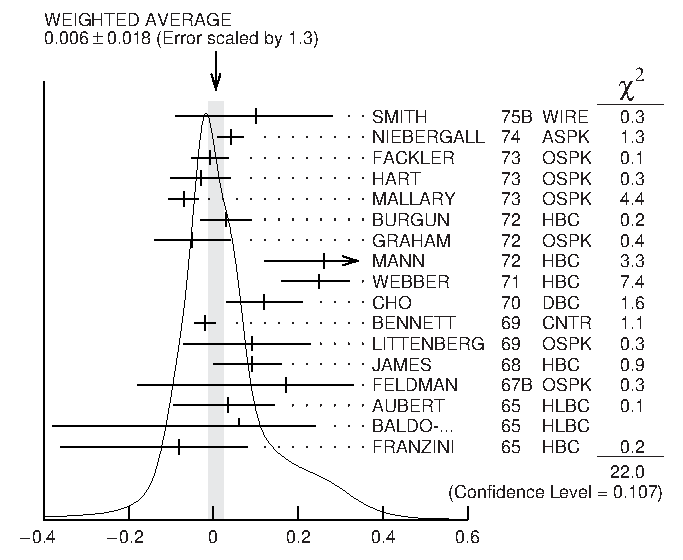
\includegraphics{filename} %multiple includegraphics may be used, 
	% with usual \hfill and \\ newline structures. 
\end{pdgxfigure}
\end{verbtex}

Figures placed in the \invt{figures} directory will be automaticallly found. 
Option keys may also be passed to individual \lstinline{\includegraphics} commands,  
as usual, if separate control is desired of multiple \lstinline{\includegraphics} in the same \invt{pdgxfigure} environment.
I.e. \lstinline!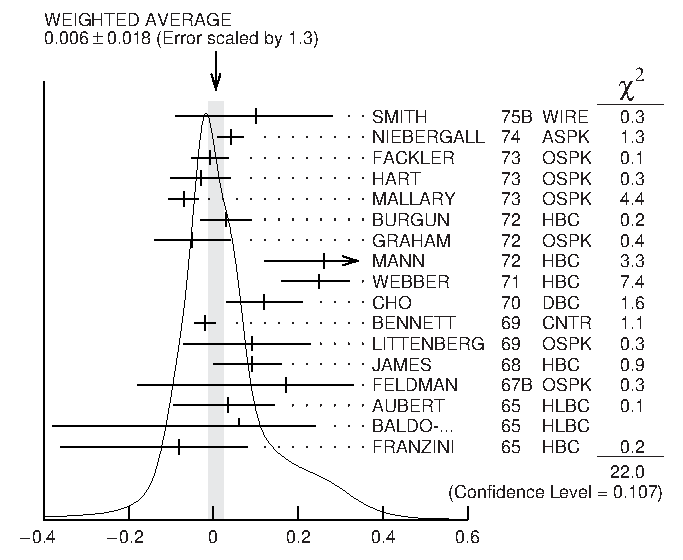
\includegraphics[<option keys>]{filename}!.

\Isubsection{Float scaling and width keys}
\label{sec:ginkeys}
As in the usual implementation of the \invt{graphicx} package, the \lstinline{\includegraphics} command takes optional standard keys \invt{width = ...}, \invt{scale = ...}.
which are used to control the width or scale of the bounding box. 
We use the same key structure to pass options to the \invt{pdgxfigure} environment, as well as to the \invt{pdgxtable} environment (see Sec.~\ref{sec:tables}).

The version specific keys \lstinline!<version>width! and \lstinline!<version>scale! have been added, 
that implement width or scaling choices only in the specific \invt{<version>}.
One may use these keys in concert with the usual \invt{width} and \invt{scale} keys, with the caveat that the order of keys matters: 
Keys are read left to right, and rightwards keys typically override leftwards ones. 
For example, passing the option keys (to either \invt{pdgxfigure} or \invt{pdgxtable}, or \lstinline{\includegraphics})
\begin{verbtex}
	[width=0.8\linewidth, bookwidth=0.9\linewidth]
\end{verbtex}
implements the \invt{width} key setting except in the book version. 
The option \lstinline!bookwidth=0.9\linewidth! followed by
\lstinline!width=0.8\linewidth! would instead implement only the version-general \lstinline!width=0.8\linewidth! setting.

\textbf{Note:} Because of specialization of the \invt{graphicx} key structure in the PDG class,
to use a \invt{scale} or \invt{<version>scale} key in an \lstinline{\includegraphics} command or \invt{pdgxfigure} environment
one must first pass an option key \invt{width=!}. This is not required for  \invt{pdgxtable}.

An additional key \lstinline!<version>bbscale! scales the float bounding box.
For some overwide floats that are larger than the nominal page width---in particular, overwide tables, see Sec.~\ref{sec:tables}---simply 
rescaling down the float does not allow it to be properly aligned on the page.
This key can be increased above $1$ (the default), to provide a sufficiently large bounding box for the float, that may then be scaled down to size with correct alignment.

\Isubsection{Available keys for \invt{pdgxfigure}}
Following is a list of available optional keys for \invt{pdgxfigure}, and default settings if not invoked.
As usual, keys are evaluated left to right. 
The version-general \invt{width} key can be used (and will override any preceeding version-specfic width key).
\begin{itemize}
	\item \invt{place}: Takes any combination of \invt{h}, \invt{t}, \invt{b}, \invt{p} (with optional \invt{\!}) that specifies float placement. Default is \invt{\!ht}.
	\item \invt{wide}: Takes \invt{true} or \invt{false} to specify the figure as full page width in either single or two column mode. Default is \invt{false}.
	\item \invt{width} or \invt{<version>width}: Sets the global or version specific width of the figure bounding box, respectively. Default is 0.75 of the line width (or text width, for wide figures).
	\item \invt{scale} or \invt{<version>scale}: Scales the figure according to float value passed to the key. 
	The option \lstinline{width=!} must be passed to turn off default width behavior and enable scaling keys.
\end{itemize}

\Isubsection{Examples}
The following produces a default-style, shown in Figure~\ref{examples:fig:example}. 
We recommend including the file extension in the \lstinline{\includegraphics} argument, to assist our editorial staff in addressing any figure quality problems.
\begin{verbtex}
\begin{pdgxfigure}[place=t] 
	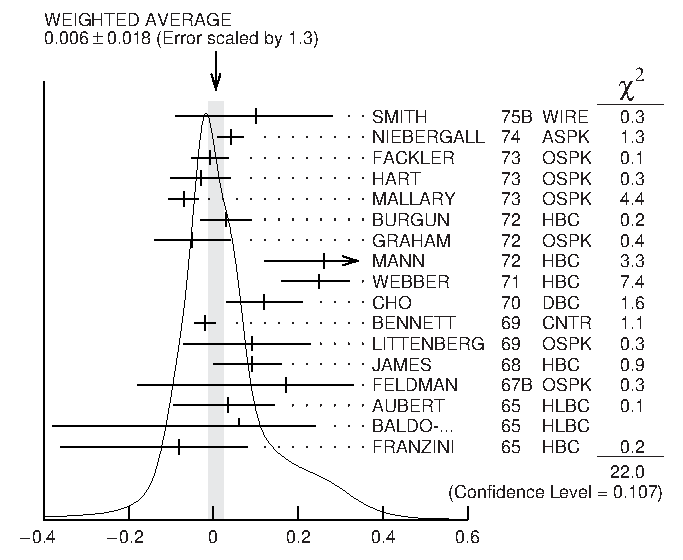
\includegraphics{filename.pdf}
	\caption{Example default figure}
	\label{examples:fig:example}
\end{pdgxfigure}
\end{verbtex}
\begin{pdgxfigure}[place=t]
	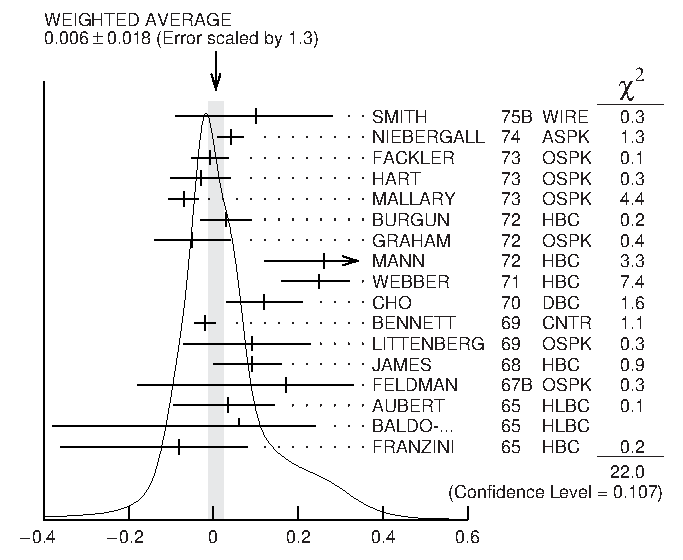
\includegraphics{filename.pdf}
	\caption{Example default figure}
	\label{examples:fig:example}
\end{pdgxfigure}

A double wide figure, shown in Fig.~\ref{examples:fig:example2}:
\begin{verbtex}
\begin{pdgxfigure}[wide=true,place=h, webwidth=0.45\linewidth, 
		bookwidth=0.9\linewidth] 
	%width key applies to all includegraphics instances
	%compiling in different versions will produce different widths
	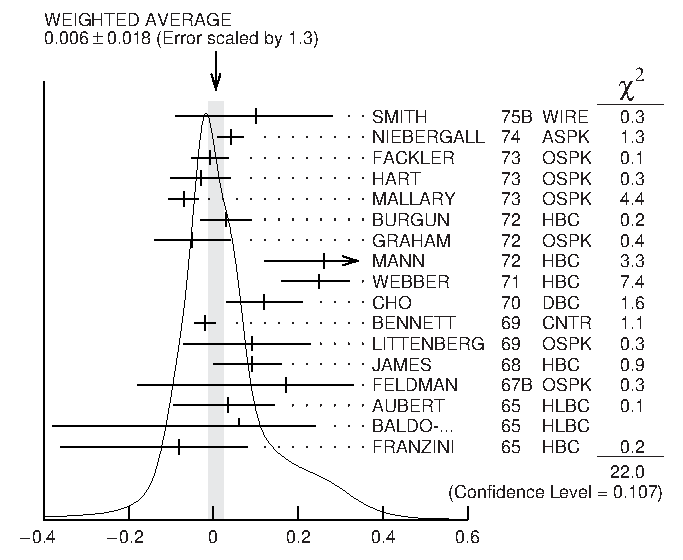
\includegraphics{filename.pdf}\hfill
	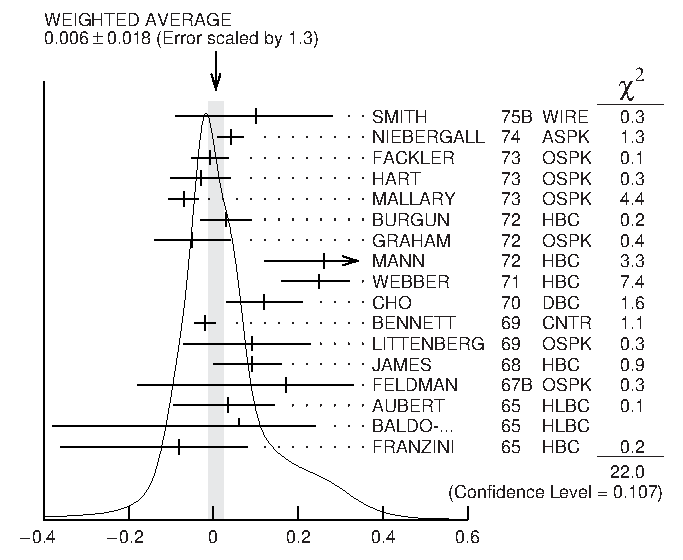
\includegraphics{filename.pdf}
	\caption{Example double wide figure, 
		with different book and web versions}
	\label{examples:fig:example2}
\end{pdgxfigure}
\end{verbtex}
\begin{pdgxfigure}[wide=true,place=h,width=0.45\textwidth] 
	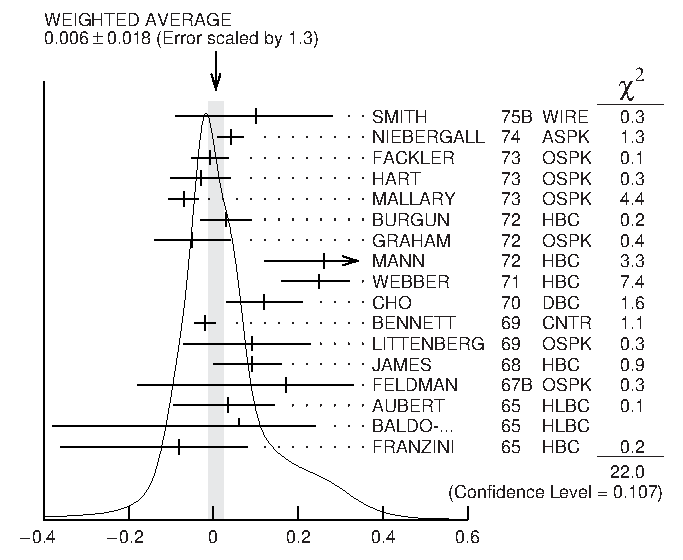
\includegraphics{filename.pdf}\hfill
	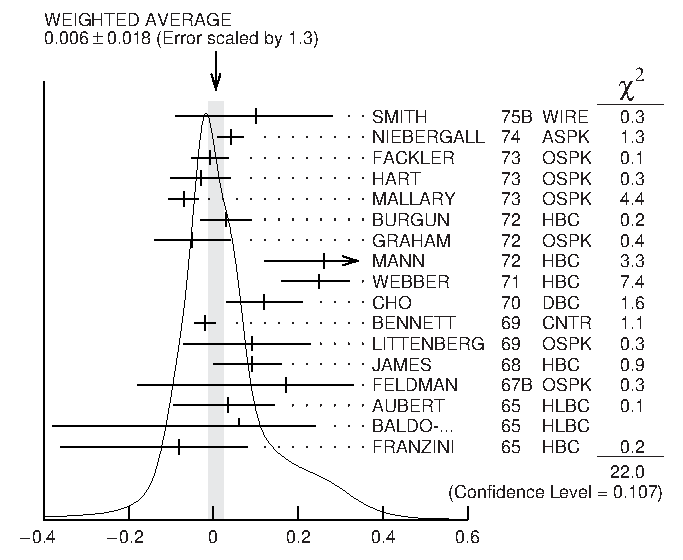
\includegraphics{filename.pdf}
	\caption{Example double wide figure, with different book and web versions}
	\label{examples:fig:example2}
\end{pdgxfigure}

A double wide figure with separate option and scaling keys, shown in Fig.~\ref{examples:fig:example3}:
\begin{verbtex}
\begin{pdgxfigure}[wide=true,place=h,width = 0.3\linewidth] 
	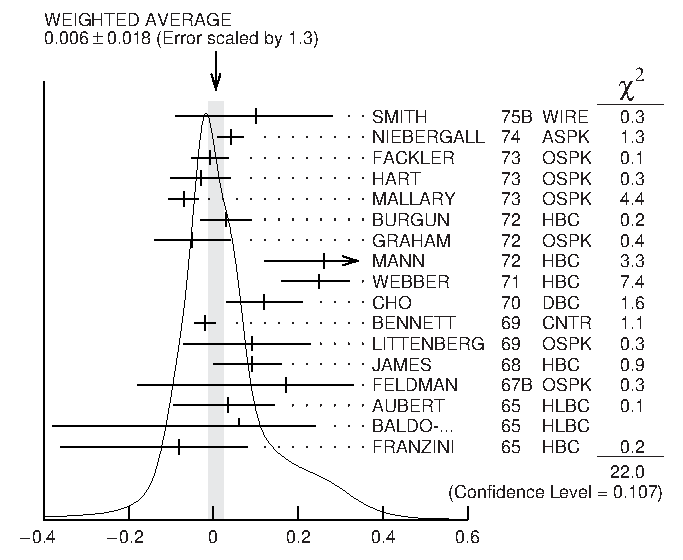
\includegraphics{filename.pdf}\hspace{1cm}
	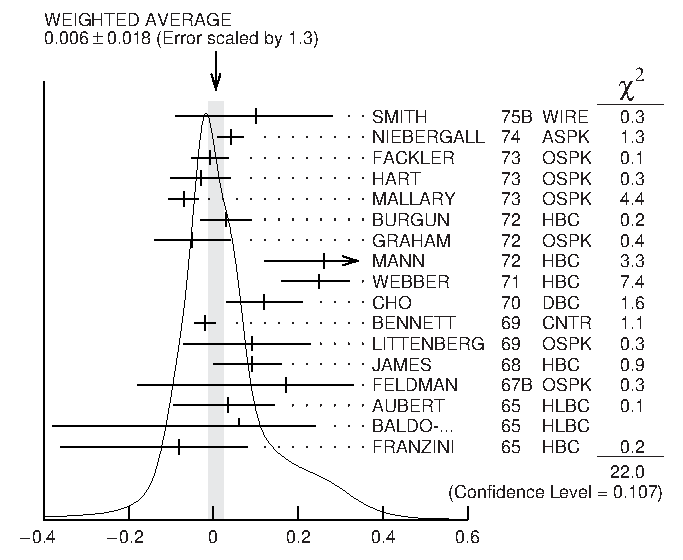
\includegraphics[width = !,scale =0.3,angle = 90]{filename}
	\caption{Example double figure, 
		with separate option and scaling keys, in both book and web versions}
	\label{examples:fig:example3}
\end{pdgxfigure}
\end{verbtex}
\begin{pdgxfigure}[wide=true,place=h,width = 0.3\linewidth] 
	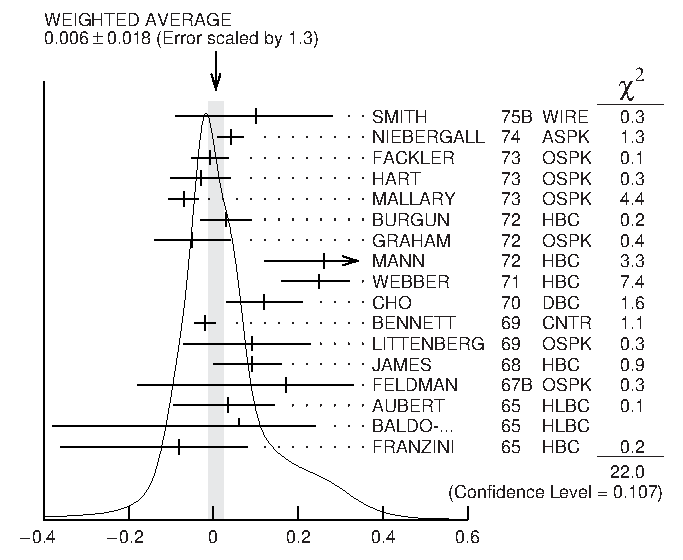
\includegraphics{filename.pdf}\hspace{1cm}
	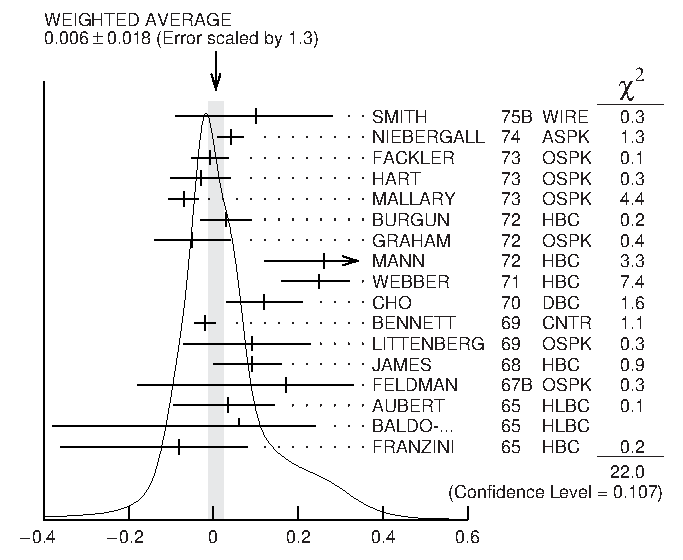
\includegraphics[width = !,scale =0.3,angle = 90]{filename}
	\caption{Example double wide figure, with separate option and scaling keys, in both book and web versions}
	\label{examples:fig:example3}
\end{pdgxfigure}

\Isubsection{\invt{pdgfigure} commands}
To add a figure, one may also use the \lstinline{\pdgfigure} or \lstinline{\pdgwidefigure} commands 
to typeset a single-column figure or double-column wide figure (for the book version), respectively. 
To include two images in one figure one may use \lstinline{\pdgdoublefigure}.
These commands are less powerful than \invt{pdgxfigure}, but automatically incorporate all PDG styles.

The macros \lstinline{\pdgfigure} and \lstinline{\pdgwidefigure} take the following arguments:
\begin{verbtex}
	\pdgfigure{<filename>}
	{<caption>}{<label>}{<placement options>}
	{<other option keys>}
\end{verbtex}
\vspace{-10pt}
while the macro \lstinline{\pdgdoublefigure} takes the following arguments:
\begin{verbtex}
	\pdgdoublefigure{<filename1>}{<filename2>}
	{<caption>}{<label>}{<placement options>}
	{<other option keys>}
\end{verbtex}
Some examples of the \invt{pdgfigure} commands are shown in Figs.~\ref{examples:fig:ideogram1}, \ref{examples:fig:ideogram2} and \ref{examples:fig:ideogram3}, respectively:
\begin{verbtex}
	\pdgfigure{filename.pdf}{Figure with caption and label}
	{examples:fig:ideogram1}{ht!}{}
	
	\pdgdoublefigure{filename.pdf}{filename.pdf}
	{Two figures, with caption and label, reduced in size}
	{examples:fig:ideogram2}{ht!}{width=0.3\textwidth}
	
	\pdgwidefigure{filename.pdf}{Wide figure}
	{examples:fig:ideogram3}{t}{}
\end{verbtex}
\FloatBarrier
\pdgfigure{filename.pdf}{Figure with caption and label}{examples:fig:ideogram1}{ht!}{}
\pdgdoublefigure{filename.pdf}{filename.pdf}{Two figures, with caption and label, reduced in size}{examples:fig:ideogram2}{ht!}{width=0.3\textwidth}
\pdgwidefigure{filename.pdf}{Wide figure}{examples:fig:ideogram3}{t}{}
\FloatBarrier

\Isection{Tables}
\label{sec:tables}
\Isubsection{ \invt{pdgxtable} and \invt{pdgxtabular}}
The PDG class provides multipurpose table and tabular environments, \invt{pdgxtable} and \invt{pdgxtabular}. 
These operate similarly to the standard \invt{table} and \invt{tabular} environments: \invt{(pdgx)table} creates a floating environment, 
while \invt{(pdgx)tabular} creates the actual tabulated display. 

The \lstinline!\caption! and \lstinline!\label! commands may be used as in the usual \invt{table} environment.
\textbf{Note: A table caption should be placed above the table.}
In addition, \invt{pdgxtable} takes a wide array of additional option keys that implement features and formatting of the prior PDG table commands/environments.  
These include keys that control placement, multicolumn spanning, version-specific widths and scaling (see Sec.~\ref{sec:ginkeys}), rotation, stretching, and caption widths.
The generic usage is
\begin{verbtex}
\begin{pdgxtable}[<option keys>]
	\caption{This is a PDG table}
	\label{tab:label}
	\begin{pdgxtabular}{<column settings>} % the usual c, l, r, | etc
		\pdgtableheader{...} %column header & separated entries go here
		%table & separated entries go here
	\end{pdgxtabular}
	%multiple pdgtabular environments are allowed
\end{pdgxtable}
\end{verbtex}

As for the usual \invt{table} environment, one may include multiple \invt{pdgxtabular}s in a single \invt{pdgxtable}.
While the \invt{pdgxtable} environment has default handling for caption widths in wide and regular tables, for both book and web versions, 
absolute control of the caption width can be implmented with a \lstinline{\captionsetup} command inside the \invt{pdgxtable} environment. 
For example \lstinline!\captionsetup{width=\linewidth}! gives a full width caption.

\Isubsection{Available keys for \invt{pdgxtable}}
Following is a list of available optional keys, and default settings if not invoked.
As usual, keys are evaluated left to right. 
While, the version-general \invt{width} key can be used (and will override any preceeding version-specfic width key), 
there is no version-general \invt{scale} key. 
Scaling of the tables is best done with the \invt{<version>scale} keys.

\begin{itemize}
	\item \invt{place}: Takes any combination of \invt{h}, \invt{t}, \invt{b}, \invt{p} (with optional \invt{\!}) that specifies float placement. Default is \invt{\!ht}.
	\item \invt{wide}: Takes \invt{true} or \invt{false} to specify the table as full page width in either single or two column mode. Default is \invt{false}.
	\item \invt{width} or \invt{<version>width}: Sets the version specific maximum width of the table bounding box. 
	Default is the maximum text width implied by the \invt{wide} key setting.
	Width settings exceeding this default are ineffective. Footnotes are scaled, but caption width is not affected.
	\item \invt{<version>scale}: Scales the table according to float value passed to the key. 
	For overwide tables, there is always a value $<1$ at which the table will be properly set to maximum page width.
	Footnotes are scaled, but caption width is not affected. Note the global \invt{scale} is disabled for \invt{pdgxtable}.
	\item \invt{<version>bbscale}: Scales the bounding box of the table. 
	For some overwide tables that are larger than the nominal page width, simply rescaling down the table does not allow the table to be properly aligned on the page.
	This key can be increased above $1$ (the default), to provide a sufficiently large bounding box for the table, that may then be scaled down to size with correct alignment.
	\item \invt{widecaptionscale}: For \invt{wide = true} tables, scales the caption width with respect to the maximum page width. Default is $0.75$.
	\item \invt{narrowcaptionscale}: For \invt{wide = false} or default tables, scales the caption width with respect to the maximum column width. Default is $0.9$.
	\item \invt{rotated}: Takes \invt{left} or \invt{right} to rotate the table, but not the caption, $90^\circ$ anticlockwise or clockwise, respectively. 
	The caption may be rotated independently, as needed with a \lstinline{\rotatebox}.
	\item \invt{sideways}: Takes \invt{true} or \invt{false} to rotate the table, including the caption, $90^\circ$ anticlockwise or clockwise, 
	according to whether the page number is even or odd.
	In a sideways table, other key width and scaling settings are still effective, but scale with respect to the page height. 
\end{itemize}


\Isubsection{Examples}
Some (simple) examples of \invt{pdgxtable} can be found in Table~\ref{examples:tab:styles} and Sec~\ref{sec:macros}.
For example, Tab.~\ref{examples:tab:styles} is typeset as
\begin{verbtex}
\begin{pdgxtable}[place=h,bookscale = 0.9,bookbbscale=2]
	\caption{Styles for the different typesetting versions}
	\label{examples:tab:styles}
	\begin{pdgxtabular}{ccccc}
		Version 		& Columns  & Font size 	& Helper Tags\footnote{
			Tags for each equation, table, figure, and bibliography entry 
			are displayed in margin or interspaced} & Line numbers\\
		\hline
		draft	& 1		   & 11pt		& Yes & Yes \\
		...
	\end{pdgxtabular}
\end{pdgxtable}
\end{verbtex}

Tables~\ref{examples:tab:commu} and~\ref{examples:tab:commp} are typeset as a two \invt{pdgxtabular}s in a single \invt{pdgxtable}, via
\begin{verbtex}
\begin{pdgxtable}[wide=true, place=!ht, webscale = 0.8]
	\caption{Common units}
	\label{examples:tab:commu}
	\begin{pdgxtabular}{lr | lr | lr}
		\showsymbol{\TeV} &  \showsymbol{\syin} & \showsymbol{\barn}   \\
		...
	\end{pdgxtabular}
	\caption{Common particles}
	\label{examples:tab:commp}
	\begin{pdgxtabular}{lr | lr | lr}
   		\showsymbol{\pp} &  \showsymbol{\ee} & \showsymbol{\pizero}   \\
  		...
	\end{pdgxtabular}
\end{pdgxtable}
\end{verbtex}

\Isubsection{Common problems and recommendations}
The \invt{pdgxtabular} environment is capable of handling the usual \lstinline{\multicolumn} and \lstinline{\multirow} objects, 
that allow for more complicated tables with cells spanning multiple rows and/or columns. 
We recommend avoiding use of \lstinline{\multispan}. 
For multiline cells, the \lstinline{\makecell} command from the \invt{makecell} package is recommended.

\Isection{Labels and referencing}
\label{sec:labels}

\Isubsection{Style guide}
As usual, the \lstinline{\label} and \lstinline{\ref} commands (and their derivatives) may be used to reference equations, tables, figures, and so on. 
To permit easy cross-referencing throughout the entire review, we request that you use the following labelling convention: \invt{BASENAME:type:name}
with \invt{type} corresponding to one of the following options
\begin{itemize}
\item {\tt fig} for figures
\item {\tt eq } for equation
\item {\tt tab} for tables
\item {\tt sec} for section, subsection etc..
\item {\tt foot} for footnotes.
\end{itemize}

\Isubsection{Missing references}

In default LaTeX, missing references are typically typeset as ``\textbf{??}''. 
To improve the typesetting experience, the \lstinline{\ref} command has been modified in the PDG class so that missing reference keys are printed out explicitly: 
For instance, a \lstinline!\ref{eqn:name}! that references a missing label called \invt{eqn:name}, will display as \ref{eqn:name}.
Similarly, the \lstinline{\cite} command will explicitly print out missing citation references. E.g. 
a \lstinline!\cite{name:2021ab}! that references a missing label called \invt{name:2021ab}, will display as \cite{name:2021ab}

\Isubsection{Cross-review referencing}
It is occasionally necessary or useful to reference (sub)sections, equations, figures, tables and so on belonging to other reviews or other reviews themselves. 
\textbf{Note:} Please use the \lstinline{\crossref} command for cross-review referencing.

Implementing a cross-reference to another review requires knowledge of its  \invt{BASENAME}:  
You must use the \invt{BASENAME} associated with the target review, not the \invt{BASENAME} of the review you're currently working on. 
To identify the  \invt{BASENAME} of another review, login into the \href{https://pdgworkspace.lbl.gov/Reviews.action}{PDG Workspace} (click to be redirected). 
Under \emph{Reviews} select from the drop-down menu \emph{All reviews}. 
Click on the title of the review you are interested in, and then select the \emph{Technical details} tab. 
The \invt{BASENAME} is the first entry.


If the full \invt{BASENAME:type:name} reference is known, you may include it with the usage \\
\lstinline!\crossref{BASENAME:type:name}!. 
This will typeset in your document as ``\crossref{BASENAME:type:name}'', because your local auxiliary files do not have the reference information of the other review.
PDG editorial staff will implement the cross-reference properly, when your review is prepared for production.

If the \invt{BASENAME:type:name} reference is not known, or the authors of the other review did not label the obect that you wish to reference, 
you may instead provide any descriptive argument to \lstinline{\crossref}. 
For example, \lstinline!\crossref{Equation 34.1.10}!.  
PDG editorial staff will implement the cross-reference properly, when your review and the other review are prepared for production.

\Isubsection{Booklet labeling and referencing}
If your review has a booklet version, it needs to be prepared at the same time as you prepare your full review.
The content to be displayed in the booklet needs to be included in \invt{BASENAME-booklet.tex}. 

The numerical tags for equations, tables, and figures in the booklet version of a review should match the tags in the full version. 
This can be achieved automatically in the booklet version by using a \lstinline!\tag{\ref{BASENAME:type:name}}! construction instead of \lstinline{\label}
to refer to the reference in the full version.
For example, if the full version has a labelled equation
\begin{verbtex}
\begin{equation}
	\label{BASENAME:eq:name}
	...
\end{equation}
\end{verbtex}
then including in \invt{BASENAME-booklet.tex}
\begin{verbtex}
\begin{equation}
	\tag{\ref{BASENAME:eq:name}}
	...
\end{equation}
\end{verbtex}
will automatically label the equation correctly. 
To achieve the same result for figures and tables, one may place in the booklet version
\begin{verbtex}
	\renewcommand{\thetable}{\ref{BASENAME:type:name}}
	\renewcommand{\thefigure}{\ref{BASENAME:type:name}}
\end{verbtex}
before each table or figure environment, respectively. 


\Isection{Index entries}
\label{sec:index}

Review authors should think about any keywords that should be included into the index of the Review of Particle Physics. PDG uses the standard \LaTeX\  \invt{makeidx} package. Thus an entry ``sample text'' can be added to the index by placing
\begin{verbtex}
\index{sample text}
\end{verbtex}
at the appropriate place in the source file. Formatting of entries with Greek letters or math symbols as well as subentries are also supported. For example
\begin{verbtex}
\index{sigma@$\$$\sigma$\$$} 
\end{verbtex}
creates an index entry $\sigma$ in the proper alphabetical order, while
\begin{verbtex}
\index{Searches!Axion searches} 
\end{verbtex}
produces a subentry ``Axion searches'' under the ``Searches'' index entry.

All index entries defined in a given review will be shown on the last page when the draft version is made. PDG staff will standardize all index entries during the final processing of all reviews. Therefore what matters is not the final formatting of index entries but that all relevant entries are added in the correct place.


\Isection{Bibliography}
\label{sec:cites}

Citations are handled using BibTeX. To add a citation to your review:
\begin{itemize}
\item Look up the reference in INSPIRE and download its BibTeX entry (see bottom of the \emph{Information} tab for the article, under \emph{Export}).
\item Add the BibTeX entry to the \invt{BASENAME.bib} file. Note the article tag assigned by INSPIRE: You can see it in the first line of the BibTeX entry, after \lstinline!@article{!.
\item Cite the reference with \lstinline{\cite}, using the article tag assigned by INSPIRE.
\end{itemize}

For example, to add a reference to the Review of Particle Physics (2018) 
add the following code to \invt{BASENAME.bib}:
\begin{verbtex}
@article{Tanabashi:2018oca,
      author         = "Tanabashi, M. and others",
      title          = "{Review of Particle Physics}",
      collaboration  = "Particle Data Group",
      journal        = "Phys. Rev.",
      volume         = "D98",
      year           = "2018",
      number         = "3",
      pages          = "030001",
      doi            = "10.1103/PhysRevD.98.030001",
      SLACcitation   = "%%CITATION = PHRVA,D98,030001;%%"
 }
\end{verbtex}
and then one may add a reference to it in \invt{BASENAME-main.tex} via \lstinline!\cite{Tanabashi:2018oca}!.

If a BibTeX entry downloaded from INSPIRE does not render correctly, 
you should first make sure you have the latest PDG style files, by running \invt{svn update} (after committing any edits you have made).
If this doesn't fix the issue please contact \invt{latexsupport@pdg.lbl.gov} for advice.  
If it appears, however, to be simply a mistake in INSPIRE's entry, 
rename the label to the form \invt{BASENAME:<INSPIRE label>} and then edit the entry as needed.
\textbf{Please do not edit entries downloaded from INSPIRE without changing the label.}
Changing the label will permit PDG editorial staff to easily identify and track edited citations, as well as notify INSPIRE of required corrections.
In case the reference does not appear in INSPIRE at all, please also use the convention for the label: \invt{BASENAME:name}.

Multiple references can be added to a single set of brackets with \lstinline!\cite{cite-key-1,cite-key-2,...}!.
One may group multiple references into the same numerical citation tag, using a \invt{*} prefix on subsequent citation keys: For example \lstinline!\cite{cite-key-1,*cite-key-2,*cite-key-3}!.
If a paper citation key is preceded by the asterisk, it can't be cited separately later, and doing so will result in a compilation error.
We recommend citing papers individually, without using the asterisk to group them.


\Isection{Footnotes}
Footnote styles are standardized throughout the review. In (rare) cases that the style needs to be changed, this is achieved via \lstinline!\setfootnotestyle{<style>}!,
where \invt{<style>} can be \lstinline{\fnsymbol} or \lstinline{\alph}, \lstinline{\Alph}, \lstinline{\arabic}, \lstinline{\roman}, \lstinline{\Roman} etc.

Sometimes the \LaTeX \ engine miscalculates the amount of space required for a footnote, resulting in overprinting of the footer.
One can help the engine obtain a better estimate by adjusting the effective page size. 
This can be done by placing \lstinline!\enlargethispage{-2\baselineskip}! somewhere just before the \lstinline{\footnote}; the \invt{-2} may be changed to any number. 

\Isection{Miscellaneous control commands}

\Isubsection{Unbalanced last page}
In the book version, the columns of the final page are automatically balanced. 
If this behavior is undesired, it may be altered by invoking \lstinline!\balancedlastpagefalse!.
The invocation may be added anywhere in the document.

\Isubsection{Blank last page}
In the book version, a blank final page may be added via \lstinline!\blankendpagetrue!.
The invocation may be added anywhere in the document.

\Isubsection{Book-only reviews}
Certain reviews are typeset for the web using the book version formatting. 
This is enforced automatically within the PDG system by \lstinline!\def\iswebbook{1}! before the \lstinline{\documentclass} invocation. 
The draft version, however, for such reviews are typeset in the usual draft/web format.

\clearpage
\Isection{PDG Macros}
\label{sec:macros}

\begin{pdgxtable}[wide=true, place=!ht, webscale = 0.8]
	\vspace{-10pt}
	\caption{Common units}
	\label{examples:tab:commu}
	\begin{pdgxtabular}{lr | lr | lr}
		\showsymbol{\TeV     } &  \showsymbol{\syin} & \showsymbol{\barn     }   \\
		\showsymbol{\MeV     } &  \showsymbol{\inch} & \showsymbol{\mbarn    }   \\
		\showsymbol{\keV     } &  \showsymbol{\ft  } & \showsymbol{\microbarn}   \\
		\showsymbol{\eV      } &  \showsymbol{\km  } & \showsymbol{\nb       }   \\
		\showsymbol{\GeVc    } &  \showsymbol{\m   } & \showsymbol{\pb       }   \\
		\showsymbol{\GeVcSq  } &  \showsymbol{\cm  } & \showsymbol{\fb       }   \\
		\showsymbol{\GeVcc   } &  \showsymbol{\mm  } & \showsymbol{\invnb    }   \\
		\showsymbol{\GeVccSq } &  \showsymbol{\mum } & \showsymbol{\invpb    }   \\
		\showsymbol{\MeVc    } &  \showsymbol{\nm  } & \showsymbol{\invfb    }   \\
		\showsymbol{\MeVcc   } &  \showsymbol{\fm  } & \showsymbol{\invab    }   \\
		\showsymbol{\invps   } &  \showsymbol{\nm  } & \showsymbol{\lum      }   \\
			&&  \showsymbol{\ma  } &&  \\
		\showsymbol{\degr    }  &  \showsymbol{\cma } && \\
			&&  \showsymbol{\mma } &&   \\
			&&  \showsymbol{\muma} &&   \\
	\end{pdgxtabular}
	\vspace{10pt}
	\caption{Common particles}
	\label{examples:tab:commp}
	\vspace{-10pt}
	\begin{pdgxtabular}{lr | lr | lr}
   \showsymbol{\pp         } &  \showsymbol{\ee           } & \showsymbol{\pizero   }   \\
   \showsymbol{\pbar       } &  \showsymbol{\epm          } & \showsymbol{\piplus   }   \\
   \showsymbol{\ppbar      } &  \showsymbol{\epem         } & \showsymbol{\piminus  }   \\
   \showsymbol{\tbar       } &  \showsymbol{\en           } & \showsymbol{\pipm     }   \\
   \showsymbol{\ttbar      } &  \showsymbol{\ep           } & \showsymbol{\pimp     }   \\
   \showsymbol{\bbar       } &  \showsymbol{\mumu         } & \showsymbol{\etaprime }   \\
   \showsymbol{\bbbar      } &  \showsymbol{\mun          } & \showsymbol{\Kzero    }   \\
   \showsymbol{\cbar       } &  \showsymbol{\mup          } & \showsymbol{\Kzerobar }   \\
   \showsymbol{\ccbar      } &  \showsymbol{\tautau       } & \showsymbol{\kaon     }   \\
   \showsymbol{\sbar       } &  \showsymbol{\taup         } & \showsymbol{\Kplus    }   \\
   \showsymbol{\ssbar      } &  \showsymbol{\taum         } & \showsymbol{\Kminus   }   \\
   \showsymbol{\ubar       } &  \showsymbol{\lepton       } & \showsymbol{\KzeroL   }   \\
   \showsymbol{\uubar      } &  \showsymbol{\leptonm      } & \showsymbol{\Kzerol   }   \\
   \showsymbol{\dbar       } &  \showsymbol{\ellm         } & \showsymbol{\Klong    }   \\
   \showsymbol{\ddbar      } &  \showsymbol{\leptonp      } & \showsymbol{\KzeroS   }   \\
   \showsymbol{\fbar       } &  \showsymbol{\ellp         } & \showsymbol{\Kzeros   }   \\
   \showsymbol{\ffbar      } &  \showsymbol{\leptonlepton } & \showsymbol{\Kshort   }   \\
   \showsymbol{\qbar       } &  \showsymbol{\ellell       } & \showsymbol{\Kstar    }   \\
   \showsymbol{\qqbar      } &  \showsymbol{\enu          } & \showsymbol{\jpsi     }   \\
   \showsymbol{\nbar       } &  \showsymbol{\munu         } & \showsymbol{\Jpsi     }   \\
   \showsymbol{\nnbar      } &  \showsymbol{\taunu        } & \showsymbol{\psip     }   \\
   \showsymbol{\neutron    } &  \showsymbol{\lnu          } & \showsymbol{\chic     }   \\
   \showsymbol{\antineutron} &  \showsymbol{\nub          } & \showsymbol{\UoneS    }   \\
   \showsymbol{\deuteron   } &  \showsymbol{\nunub        } & \showsymbol{\chib     }   \\
   \showsymbol{\Zzero      } &  \showsymbol{\nue          } & \showsymbol{\Dstar    }   \\
   \showsymbol{\Zboson     } &  \showsymbol{\nueb         } & \showsymbol{\Bd       }   \\
   \showsymbol{\Wplus      } &  \showsymbol{\nuenueb      } & \showsymbol{\Bs       }   \\
   \showsymbol{\Wminus	   } &  \showsymbol{\num          } & \showsymbol{\Bu       }   \\
   \showsymbol{\Wboson	   } &  \showsymbol{\numb         } & \showsymbol{\Bc       }   \\ 
   \showsymbol{\Wpm   	   } &  \showsymbol{\numnumb      } & \showsymbol{\Lb       }   \\
   \showsymbol{\Wmp        } &  \showsymbol{\nut          } & \showsymbol{\Bstar    }   \\
   \showsymbol{\Hzero } &  \showsymbol{\nutb         } & \showsymbol{\BoBo     }   \\
   \showsymbol{\Hboson}  &	\showsymbol{\nutnutb      } & \showsymbol{\BodBod   }    \\		    
   \showsymbol{            } &	\showsymbol{              } & \showsymbol{\BosBos   }    \\		    
   \showsymbol{            } &	\showsymbol{              } & \showsymbol{\LambdaStar}  \\
	\end{pdgxtabular}
\end{pdgxtable}

\begin{pdgxtable}[wide=true, place=h, webscale = 0.8]
	\caption{Hypothetical particles}
	\begin{pdgxtabular}{lr | lr | lr}
   \showsymbol{\Azero }      &  \showsymbol{\gravino   } & \showsymbol{\slepton   }   \\
   \showsymbol{\hzero }      &  \showsymbol{\Zprime    } & \showsymbol{\sleptonL  }   \\
   \showsymbol{\Hzero }      &  \showsymbol{\Zstar     } & \showsymbol{\sleptonR  }   \\
   \showsymbol{\Hplus }  	  &  \showsymbol{\squark    } & \showsymbol{\sel       }   \\
   \showsymbol{\Hminus}       &  \showsymbol{\squarkL   } & \showsymbol{\selL      }   \\
   \showsymbol{\Hpm   }   	&  \showsymbol{\squarkR   } & \showsymbol{\selR      }   \\
   \showsymbol{\Hmp   }       &  \showsymbol{\gluino    } & \showsymbol{\smu       }   \\
   \showsymbol{\ggino }     &  \showsymbol{\stop      } & \showsymbol{\smuL      }   \\
   \showsymbol{\chinop}      &  \showsymbol{\stopone   } & \showsymbol{\smuR      }   \\
   \showsymbol{\chinom}      &  \showsymbol{\stoptwo   } & \showsymbol{\stau      }   \\
   \showsymbol{\chinopm}      &  \showsymbol{\stopL     } & \showsymbol{\stauL     }   \\
   \showsymbol{\chinomp}     &  \showsymbol{\stopR     } & \showsymbol{\stauR     }   \\
   \showsymbol{\chinoonep}     &  \showsymbol{\sbottom   } & \showsymbol{\stauone   }   \\
   \showsymbol{\chinoonem}   &  \showsymbol{\sbottomone} & \showsymbol{\stautwo   }   \\
   \showsymbol{\chinoonepm}   &  \showsymbol{\sbottomtwo} & \showsymbol{\snu       }   \\
   \showsymbol{\chinotwop}  &  \showsymbol{\sbottomL  } & \showsymbol{           }   \\
   \showsymbol{\chinotwom}   &  \showsymbol{\sbottomR  } & \showsymbol{           }   \\
   \showsymbol{\chinotwopm}   &  \showsymbol{           } & \showsymbol{           }   \\
   \showsymbol{\nino}  &  \showsymbol{           } & \showsymbol{           }   \\
   \showsymbol{\ninoone}        &  \showsymbol{           } & \showsymbol{           }   \\
   \showsymbol{\ninotwo}     &  \showsymbol{           } & \showsymbol{           }   \\
   \showsymbol{\ninothree}     &  \showsymbol{           } & \showsymbol{           }   \\
   \showsymbol{\ninofour}   &  \showsymbol{           } & \showsymbol{           }   \\
	\end{pdgxtabular}
\vspace*{10pt}
	\caption{Useful symbols for proton-proton physics}
\vspace*{-10pt}	
	\begin{pdgxtabular}{lr | lr }
   \showsymbol{\pT  }      &  \showsymbol{\rts }   \\
   \showsymbol{\pt  }      &  \showsymbol{\sqs } \\
   \showsymbol{\ET  }      &  \showsymbol{\mh}  \\
   \showsymbol{\eT  }      &  \showsymbol{\mW}  \\
   \showsymbol{\et  }      & \showsymbol{\mZ}   \\
   \showsymbol{\HT  }      & \showsymbol{\mH}   \\
   \showsymbol{\pTsq}      &&   \\
   \showsymbol{\MET }      &&   \\
   \showsymbol{\met }      &&   \\
   \showsymbol{\Ecm }      &&   \\
	\end{pdgxtabular}
\vspace*{10pt}
	\caption{Monte Carlo Generators}
\vspace*{-10pt}		
	\begin{pdgxtabular}{lr | lr | lr}	
   \showsymbol{\ACERMC    }      &  \showsymbol{\MCatNLO   } & \showsymbol{\Comphep    }   \\
   \showsymbol{\ALPGEN    }      &  \showsymbol{\AMCatNLO  } & \showsymbol{\Prospino   }   \\
   \showsymbol{\GEANT     }      &  \showsymbol{\MCFM      } & \showsymbol{\LO         }   \\
   \showsymbol{\Herwigpp  }      &  \showsymbol{\METOP     } & \showsymbol{\NLO        }   \\
   \showsymbol{\HERWIGpp  }      &  \showsymbol{\POWHEG    } & \showsymbol{\NLL        }   \\
   \showsymbol{\Herwig    }      &  \showsymbol{\POWHEGBOX } & \showsymbol{\NNLO       }   \\
   \showsymbol{\HERWIG    }      &  \showsymbol{\POWPYTHIA } & \showsymbol{\muF        }   \\
   \showsymbol{\JIMMY     }      &  \showsymbol{\PROTOS    } & \showsymbol{\muR        }   \\
   \showsymbol{\MADSPIN   }      &  \showsymbol{\PYTHIA    } & \showsymbol{            }   \\
   \showsymbol{\MADGRAPH  }      &  \showsymbol{\SHERPA    } & \showsymbol{            }   \\
   \showsymbol{\MGMCatNLO }      &  \showsymbol{           } & \showsymbol{            }   \\
	\end{pdgxtabular}
\end{pdgxtable}

\Isection{Tables: Legacy commands}

Though no longer recommended, legacy \lstinline{\pdgtable} or \lstinline{\pdgwidetable} commands 
to typeset a single-column table or double-column wide table (for the book version), respectively.
The \lstinline{\pdgtableheader} macro may be used in the first line of the table to automatically typeset a header.

The macros \lstinline{\pdgtable} and \lstinline{\pdgwidetable} take the following arguments:
\begin{verbtex}
	\pdgtable{<column styles>}
	{<caption>}{<label>}{<option keys>}
\end{verbtex}
Some examples usages of these commands follow, in Tables~\ref{examples:tab:table1}, \ref{examples:tab:table2} and~\ref{examples:tab:table3} below.
\begin{verbtex}
\begin{pdgtable}{c c c} 
	{Table}{examples:tab:table1}{h!}
	\pdgtableheader{ Column 1 & Column 2 & Column 3}
	row1  & 1  & 2\\
	row2  & 1  & 2\\
	row3  & 1  & 2\\
\end{pdgtable}
\end{verbtex}   
\begin{verbtex}
\begin{pdgtable}{|c | c | c | c|} 
	{Multicolumn table}{examples:tab:table2}{h!}
	\pdgtableheader{ \multicolumn{2}{c}{Column 1} & 
	\multicolumn{2}{c}{Column 2}}
	\pdgtableheader{ A & B& C & D }
	row1  & 1 & 2 &3 \\
	row2  & 1 & 2 &3 \\
\end{pdgtable}
\end{verbtex}  
\begin{verbtex}
\begin{pdgtable}{c l}
	{Table with footnotes}{examples:tab:table3}{}
	One value & another\footnote{This is something to notice
	\label{kmmix:foot:one}}\\
	Two values\footref{kmmix:foot:one} & another \\
\end{pdgtable}
\end{verbtex} 
 
\FloatBarrier 
\begin{pdgtable}{c c c} 
{Table}{examples:tab:table1}{h!}
\pdgtableheader{ Column 1 & Column 2 & Column 3}
row1  & 1  & 2\\
row2  & 1  & 2\\
row3  & 1  & 2\\
\end{pdgtable}
\begin{pdgtable}{|c | c | c | c|} 
{Multicolumn table}{examples:tab:table2}{h!}
\pdgtableheader{ \multicolumn{2}{|c|}{Column 1} & 
\multicolumn{2}{|c|}{Column 2}}
\pdgtableheader{ A & B& C & D }
row1  & 1 & 2 &3 \\
row2  & 1 & 2 &3 \\
\end{pdgtable}
\begin{pdgtable}{c l}
{Table with footnotes}{examples:tab:table3}{}
One value & another\footnote{This is something to notice\label{kmmix:foot:one}}\\
Two values\footref{kmmix:foot:one} & another \\
\end{pdgtable}
! line that includes these instructions in the main source file of your review, \invt{databases-main.tex}.

This documentation focuses mostly on the specialized functionality of the PDG \LaTeX \ class: %There are many resources that provide more general guidance for typesetting in \LaTeX.
For further support, or any \LaTeX-related questions, we invite authors to contact
\vspace{-0.2cm}
\begin{center}
\scalebox{1.5}{
	\invt{latexsupport@pdg.lbl.gov}
}
\end{center}

\Isubsection{File structure}
The source files for a PDG review are kept in separate directories within a SVN repository. 
Some files in each directory are auto-generated, while others are designed to be edited by review authors. 
\textbf{Do not edit auto-generated files, as any edits to these files will be overwritten periodically.}

Each review is assigned a unique name ("basename") that is used to label the relevant review files and will be referred to as \invt{BASENAME} in the following. For example, the QCD review is assigned basename \invt{qcd}. Therefore \invt{BASENAME-main.tex} in this documentation refers to file \invt{qcd-main.tex} for the QCD review.

Your review is assigned basename \invt{databases}.

The basename is further used to label cross-references to the review (see Sec.~\ref{sec:labels}) and specialized citations (see Sec.~\ref{sec:cites}). 
The file structure of a typical review is as follows:
\begin{itemize}
\item \invt{BASENAME-main.tex} --- contains the text of your review. 
\item \invt{BASENAME-booklet.tex} --- contains the text of the booklet version of your review (if there is one)
\item \invt{BASENAME-preamble.tex} --- contains review-specific definitions or inclusion of packages, that need to go into the document's preamble
\item \invt{BASENAME.bib} --- BibTeX bibliography entries (see Sec~\ref{sec:cites})
\item \invt{/figures} --- directory containing all figures
\item Auxiliary files (\invt{.aux}, \invt{.out}, \invt{.log}) --- these are generated by the \LaTeX compiler
\item Other \invt{.tex} files --- may be added and included in \invt{BASENAME-main.tex} or \invt{BASENAME-booklet.tex} with the \lstinline{\input} command.
\item \textbf{[auto-generated]} \invt{BASENAME.tex} --- compilation file for the review
\item \textbf{[auto-generated]} \invt{Makefile} --- Makefile to compile the review automatically (see Sec.~\ref{sec:make})
\item \textbf{[auto-generated]} \invt{pdg.cls} --- PDG \LaTeX \ class file
\item \textbf{[auto-generated]} \invt{pdg.bst} --- BibTeX PDG style file
\item \textbf{[auto-generated]} \invt{pdg-xr-hyper.sty} --- helper BibTeX style file
\item \textbf{[auto-generated]} \invt{pdgdefs.tex} --- PDG standard symbols and macros
\item \textbf{[auto-generated]} \invt{examples.tex} --- This file
\end{itemize}

\begin{center}
~\\
%!%\vspace{-12pt}
%!%In your review, the basename is databases.
\end{center}
To identify the  \invt{BASENAME} of yours or another review, you may also login into the 
\href{https://pdgworkspace.lbl.gov/Reviews.action}{PDG Workspace} (click to be redirected). 
Under \emph{Reviews} select from the drop-down menu \emph{All reviews}. 
Click on the title of the review you are interested in, and then select the \emph{Technical details} tab. 
The \invt{BASENAME} is the first entry.

\Isubsection{Multiversion typesetting}
The PDG \LaTeX \ class has functionality to typeset in four different versions or styles: draft, web, book and booklet. 
(The draft and web versions are referred to below jointly as `web', since they are broadly similar). 
See Table~\ref{examples:tab:styles} for a broad summary.

\begin{pdgxtable}[place=h,bookscale = 0.9,bookbbscale=2]
	\caption{Styles for the different typesetting versions}
	\label{examples:tab:styles}
	\begin{pdgxtabular}{ccccc}
		Version 		& Columns  & Font size 	& Helper Tags\footnote{
			Tags for each equation, table, figure, and bibliography entry are displayed in margin or interspaced} & Line numbers\\
		\hline
		\invt{draft} 	& 1		   & 11pt		& Yes & Yes \\
		\invt{web} 		& 1		   & 11pt		& No  & No\\
		\invt{book} 	& 2		   & 8pt		& No  & No\\
		\invt{booklet} 	& 1		   & 8pt		& No & No \\
	\end{pdgxtabular}
\end{pdgxtable}

Specialized macros may also have version-specific implementations. 
These follow the naming convention \invt{<version><macroname>}, where \invt{<version>} may take values of \invt{book}, \invt{booklet} and \invt{web}.
See for example, Sec.~\ref{sec:align}.
Specialized option keys follow the same convention. See e.g. Sec.~\ref{sec:ginkeys}.


\Isubsection{Makefile}
\label{sec:make}
We recommend to compile the review using \invt{make} on the command line. The usage is as follows:
\begin{itemize}
	\item \invt{make} --- compiles in draft mode.
	\item \invt{make  <version>} --- compiles in \invt{<version>} mode. For example \invt{make web}.
	\item \invt{make bib} --- compiles only the BibTeX files.
	\item \invt{make clean} --- cleans out all auxiliary files.
	\item \invt{make cleanall} --- cleans out the compiled pdf and all auxiliary files.
	\item \invt{make prod} --- cleans all auxiliary files, then compiles the web version.
	\item {\footnotesize{\texttt{make crossref}}} --- compiles required cross-referencing files (advanced: requires checkout of the other reviews to be cross-referenced).
\end{itemize}



\Isection{Style guides}
\Isubsection{Particle symbols}
Particle symbols are italic (or slanted) characters: \en, \pbar, \Lb, \pizero, \Klong, \Dstar. 
Charge is indicated by a superscript: $B^{-}$, $\Delta^{++}$. 
Charge is not normally indicated for $p$, $n$, or the quarks, and is optional for neutral isosinglets: $\eta$ or $\eta^{0}$. 
Antiparticles and particles are distinguished by charge for
charged leptons and mesons: $\tau^{+}$, $\kaon^{-}$ 
Otherwise, distinct antiparticles are indicated by a bar (overline): $\nbar_{\mu}$, \tbar, \pbar, \Kzerobar.

\Isubsection{Macros and shortcuts}
The \invt{pdgdefs.tex} file implements a series of useful macros for particle symbols, units and other common notation. 
All definitions are terminated with  \lstinline!\string\xspace!, so you can simply write ``\lstinline!\ttbar production!'' to typeset inline ``\ttbar production''.
The entire list of macros is provided in Sec.~\ref{sec:macros}.

Most Monte Carlo generators have a macro with a suffix 'V' that allows you to include the version. E.g. \lstinline!\PYTHIAV{8.1}! produces \PYTHIAV{8.1}.
In case you need to define other symbols, please add them to the \invt{BASENAME-preamble.tex} file.

\Isubsection{Column switching}

The web version is typeset as single column, singleside 11pt style, the book as 8pt double column, double sided.

In all versions of the review, switching between single and double column mode can be done \emph{in situ} with \lstinline{\onecolumn} or \lstinline{\twocolumn}
respectively. For example

\medskip
\ifrppbook
	\onecolumn
\else
	\twocolumn
\fi
{\footnotesize{Lorem ipsum dolor sit amet, consectetur adipiscing elit. Duis congue lectus at lectus tristique porta. Vivamus scelerisque porta massa, laoreet pulvinar dolor blandit vitae. Nam rhoncus id risus in tincidunt. Maecenas ultrices, arcu id gravida tempor, urna libero sodales nunc, quis dapibus ipsum quam eget est. Quisque eget convallis odio, at pellentesque quam. Mauris pretium eu metus ac imperdiet. Class aptent taciti sociosqu ad litora torquent per conubia nostra, per inceptos himenaeos. Nulla quis tincidunt libero. Aliquam posuere at quam quis posuere. Etiam turpis nulla, faucibus eget massa sagittis, porttitor sagittis elit. Proin a lorem eleifend, rhoncus orci quis, mattis metus. Donec sit amet lobortis lacus. Quisque magna augue, elementum nec ipsum non, feugiat ultricies urna. Sed tincidunt nisl vestibulum leo finibus, vitae sollicitudin sapien bibendum. Duis maximus ipsum nec urna lobortis, sed scelerisque nulla facilisis. Sed id finibus libero. }}
\ifrppbook
	\twocolumn
\else
	\onecolumn
\fi
\medskip

\Isection{Equations}
Equations may be typeset using the \invt{equation}, \invt{array}, \invt{multline}, and \invt{gather} etc environments provided by \invt{amsmath} package. 
We do not recommend using \invt{eqnarray}. As a trivial example
\begin{verbtex}
\begin{equation}
\label{BASENAME:eq:equation}
	N_{exp} = \sigma_{exp} \times \int L(t) dt
\end{equation}
\end{verbtex}
which produces
\begin{equation}
	N_{exp} = \sigma_{exp} \times \int L(t) dt
\end{equation}


To tag a set of equations with a common numbering and label, please use the \invt{subequation} environment, together with \invt{align}.
As an example:
\begin{verbtex}
\begin{subequations}
	\label{BASENAME:eq:equation1}
	\begin{align}
		A + B = C\\
		D= \frac{E}{F}  
	\end{align}
\end{subequations}
\end{verbtex}
which produces
\begin{subequations}
\begin{align}
	A + B = C\\
	D= \frac{E}{F}  
\end{align}
\end{subequations}


\Isubsection{Wide equations: \invt{pdgstrip}}
Some wide equations are not easily amenable to display in the PDG book double column format. 
Similar to the ReVTeX \invt{widetext} environment, the PDG style provides a \invt{pdgstrip} environment, that may wrap any other equation (or align, array etc) environment. 
The \invt{pdgstrip} environment is not a float, and will respect absolute placement in the typesetting stream. 
For example:
\begin{verbtex}
	\begin{pdgstrip}
		\begin{equation} % or any other display environment
		...

		\end{equation}
	\end{pdgstrip}
\end{verbtex}
In the web and booklet versions, this environment performs no operation on the wrapped environment. 
In the book version, the equation is preserved as a single `strip' across both columns, with column-wide rules to guide the reader's eye. 
The column-wide rules may be disabled -- e.g if the strip environment falls at the top or bottom of a page --  by passing the option \invt{plain} to the \invt{pdgstrip} environment. I.e. 
\lstinline!\begin{pdgstrip}[plain]!.

In principle, the pdgstrip envirornment may also wrap a floating environment such as a figure. 
In the book version, this will disable the ability of the figure to float, and fix it to a desired location.

\Isubsection{Alignment}
\label{sec:align}
Within \invt{align} environments or any other environment that uses the special \invt{&} and \invt{\\\\} (or \lstinline{\cr}) control characters for alignment, one may use
use version specific \lstinline!\bookalign!, \lstinline!\webalign!, \lstinline!\bookletalign! and \lstinline!\bookcr!, \lstinline!\webcr!, \lstinline!\bookletcr! macros.

The \lstinline!\<version>align! macros insert a `\invt{&}' control character only in the \invt{<version>} of the review. 
The \lstinline!\<version>cr! macro similarly inserts a carriage return `\invt{\\\\}' only in the \invt{<version>} of the review, 
but takes two additional arguments that are placed before and after the carriage return, respectively. For instance,
\lstinline!\bookcr{\nonumber}{[10pt]}! inserts \lstinline!\nonumber\\[10pt]!.  An example usage is
\begin{verbtex}
\begin{align}
	{\cal A}_f 
	\bookalign = \frac{\Gamma(\bar{B}^0(t) \to f) - \Gamma(B^0(t) \to f)}
		{\Gamma(\bar{B}^0(t) \to f) + \Gamma(B^0(t) \to f)} \bookcr{\,,\nonumber}{}
	\bookalign = S_f \sin(\Delta m_d\, t) - C_f \cos(\Delta m_d\, t) \,.
\end{align}
\end{verbtex}
This produces in the web version
\ifrppbook
\onecolumn
	\begin{align}
		{\cal A}_f  = \frac{ \Gamma(\bar{B}^0(t) \to f) - \Gamma(B^0(t) \to  f) }
			{ \Gamma(\bar{B}^0(t) \to f) + \Gamma(B^0(t) \to  f) } 
			= S_f \sin(\Delta m_d\, t) - C_f \cos(\Delta m_d\, t) \,,
	\end{align}
\twocolumn
\else
	\begin{align}
		{\cal A}_f 
		\bookalign = \frac{ \Gamma(\bar{B}^0(t) \to f) - \Gamma(B^0(t) \to  f) }
			{ \Gamma(\bar{B}^0(t) \to f) + \Gamma(B^0(t) \to  f) } \bookcr{\,,\nonumber}{}
		\bookalign = S_f \sin(\Delta m_d\, t) - C_f \cos(\Delta m_d\, t) \,,
	\end{align}
\fi	
and in the two column book version
\addtocounter{equation}{-1}
\ifrppweb
	\twocolumn
	\begin{align}
		{\cal A}_f 
		& = \frac{ \Gamma(\bar{B}^0(t) \to f) - \Gamma(B^0(t) \to  f) }
			{ \Gamma(\bar{B}^0(t) \to f) + \Gamma(B^0(t) \to  f) } \,,\nonumber\\
		& = S_f \sin(\Delta m_d\, t) - C_f \cos(\Delta m_d\, t) \,,
	\end{align}
	\onecolumn
\else
	\begin{align}
		{\cal A}_f 
		\bookalign = \frac{ \Gamma(\bar{B}^0(t) \to f) - \Gamma(B^0(t) \to  f) }
			{ \Gamma(\bar{B}^0(t) \to f) + \Gamma(B^0(t) \to  f) } \bookcr{\,,\nonumber}{}
		\bookalign = S_f \sin(\Delta m_d\, t) - C_f \cos(\Delta m_d\, t) \,,
	\end{align}
\fi

\Isection{Figures}

\Isubsection{Figure requirements}
Permitted figure formats (for pdflatex) are pdf, png and jpg, in order of preferred format. 
In addition, please note:
\begin{itemize}
	\item Submissions should be be provided with a minimum resolution of 150DPI. However, 300DPI or greater is preferred.
	\item Our preference for the submission color palette is CMYK, but RGB is acceptable.
	\item Visible line (stroke) weight must be no less than $0.5$px, preferably at least $1$px.
	\item Submissions should be provided with fonts embedded, if possible.
	\item In print, colors are often not as vibrant or saturated as they appear on screen. Therefore, overlapping areas of color should be high contrast for visual clarity: 
	e.g. do not place magenta over blue, or light blue over a light green.	
\end{itemize}
If you are unsure your figure is of sufficient resolution or quality, please contact \invt{latexsupport@pdg.lbl.gov} for advice.

Encapsulated postscript or postscript figures may also be used, but they require conversion to pdf. 
Depending on your \LaTeX \ engine settings, running \invt{pdflatex} may automatically convert eps or ps files. 
If not, the conversion can be done manually with various programs, such as ImageMagick, or \invt{epstopdf} and \invt{pstopdf}.

\textbf{Note:} Make sure that the figure file is added into the subdirectory \invt{figures}, and that it is commited to svn or provided with your text.

\Isubsection{\invt{pdgxfigure} environment}
The multipurpose figure environment \invt{pdgxfigure} is now available, as an alternative to the various \invt{pdgfigure} and related commands.
These operate similarly to the standard \invt{figure} environments: \invt{(pdgx)figure} creates a floating environment.

The \lstinline!\caption! and \lstinline!\label! commands may be used as in the usual \invt{figure} environment. 
\textbf{Note: A figure caption should be placed below the figure.}
In addition, \invt{pdgxfigure} takes an array of additional option keys that implement features and formatting of the prior PDG figure commands.
These include keys that control placement, multicolumn spanning, and version-specific widths. 
The generic usage is
\begin{verbtex}
\begin{pdgxfigure}[<option keys>]
	\caption{This is a PDG figure}
	\label{examples:fig:label}
	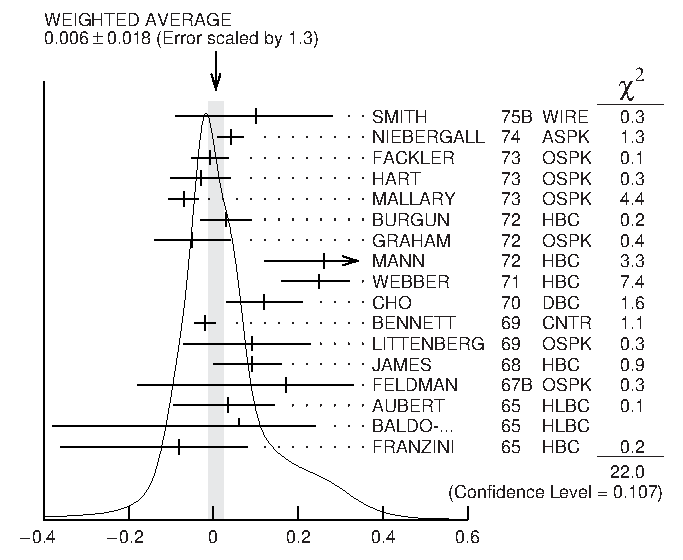
\includegraphics{filename} %multiple includegraphics may be used, 
	% with usual \hfill and \\ newline structures. 
\end{pdgxfigure}
\end{verbtex}

Figures placed in the \invt{figures} directory will be automaticallly found. 
Option keys may also be passed to individual \lstinline{\includegraphics} commands,  
as usual, if separate control is desired of multiple \lstinline{\includegraphics} in the same \invt{pdgxfigure} environment.
I.e. \lstinline!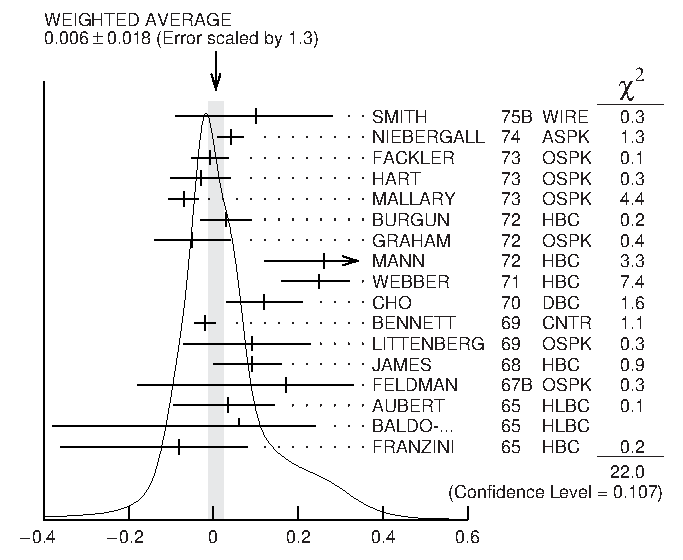
\includegraphics[<option keys>]{filename}!.

\Isubsection{Float scaling and width keys}
\label{sec:ginkeys}
As in the usual implementation of the \invt{graphicx} package, the \lstinline{\includegraphics} command takes optional standard keys \invt{width = ...}, \invt{scale = ...}.
which are used to control the width or scale of the bounding box. 
We use the same key structure to pass options to the \invt{pdgxfigure} environment, as well as to the \invt{pdgxtable} environment (see Sec.~\ref{sec:tables}).

The version specific keys \lstinline!<version>width! and \lstinline!<version>scale! have been added, 
that implement width or scaling choices only in the specific \invt{<version>}.
One may use these keys in concert with the usual \invt{width} and \invt{scale} keys, with the caveat that the order of keys matters: 
Keys are read left to right, and rightwards keys typically override leftwards ones. 
For example, passing the option keys (to either \invt{pdgxfigure} or \invt{pdgxtable}, or \lstinline{\includegraphics})
\begin{verbtex}
	[width=0.8\linewidth, bookwidth=0.9\linewidth]
\end{verbtex}
implements the \invt{width} key setting except in the book version. 
The option \lstinline!bookwidth=0.9\linewidth! followed by
\lstinline!width=0.8\linewidth! would instead implement only the version-general \lstinline!width=0.8\linewidth! setting.

\textbf{Note:} Because of specialization of the \invt{graphicx} key structure in the PDG class,
to use a \invt{scale} or \invt{<version>scale} key in an \lstinline{\includegraphics} command or \invt{pdgxfigure} environment
one must first pass an option key \invt{width=!}. This is not required for  \invt{pdgxtable}.

An additional key \lstinline!<version>bbscale! scales the float bounding box.
For some overwide floats that are larger than the nominal page width---in particular, overwide tables, see Sec.~\ref{sec:tables}---simply 
rescaling down the float does not allow it to be properly aligned on the page.
This key can be increased above $1$ (the default), to provide a sufficiently large bounding box for the float, that may then be scaled down to size with correct alignment.

\Isubsection{Available keys for \invt{pdgxfigure}}
Following is a list of available optional keys for \invt{pdgxfigure}, and default settings if not invoked.
As usual, keys are evaluated left to right. 
The version-general \invt{width} key can be used (and will override any preceeding version-specfic width key).
\begin{itemize}
	\item \invt{place}: Takes any combination of \invt{h}, \invt{t}, \invt{b}, \invt{p} (with optional \invt{\!}) that specifies float placement. Default is \invt{\!ht}.
	\item \invt{wide}: Takes \invt{true} or \invt{false} to specify the figure as full page width in either single or two column mode. Default is \invt{false}.
	\item \invt{width} or \invt{<version>width}: Sets the global or version specific width of the figure bounding box, respectively. Default is 0.75 of the line width (or text width, for wide figures).
	\item \invt{scale} or \invt{<version>scale}: Scales the figure according to float value passed to the key. 
	The option \lstinline{width=!} must be passed to turn off default width behavior and enable scaling keys.
\end{itemize}

\Isubsection{Examples}
The following produces a default-style, shown in Figure~\ref{examples:fig:example}. 
We recommend including the file extension in the \lstinline{\includegraphics} argument, to assist our editorial staff in addressing any figure quality problems.
\begin{verbtex}
\begin{pdgxfigure}[place=t] 
	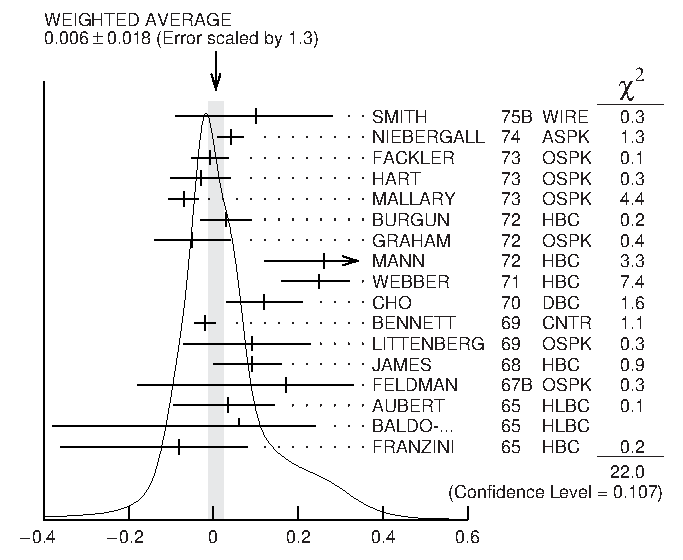
\includegraphics{filename.pdf}
	\caption{Example default figure}
	\label{examples:fig:example}
\end{pdgxfigure}
\end{verbtex}
\begin{pdgxfigure}[place=t]
	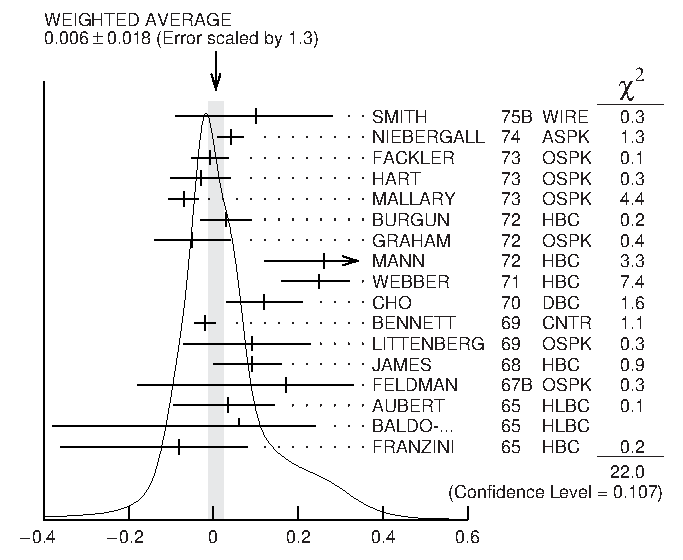
\includegraphics{filename.pdf}
	\caption{Example default figure}
	\label{examples:fig:example}
\end{pdgxfigure}

A double wide figure, shown in Fig.~\ref{examples:fig:example2}:
\begin{verbtex}
\begin{pdgxfigure}[wide=true,place=h, webwidth=0.45\linewidth, 
		bookwidth=0.9\linewidth] 
	%width key applies to all includegraphics instances
	%compiling in different versions will produce different widths
	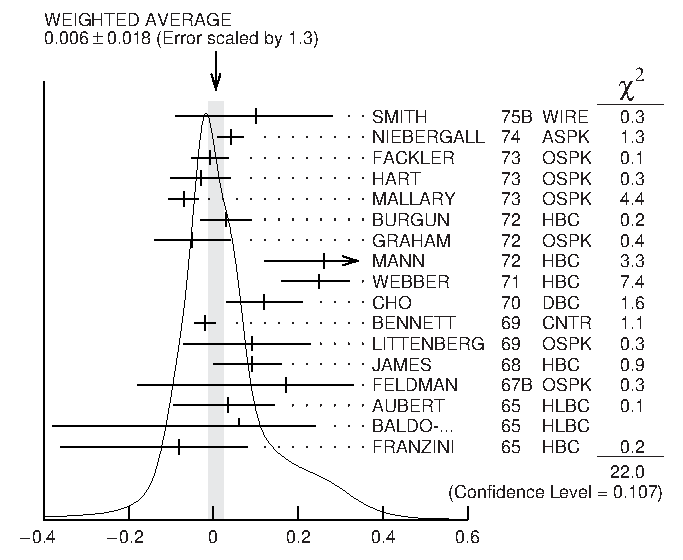
\includegraphics{filename.pdf}\hfill
	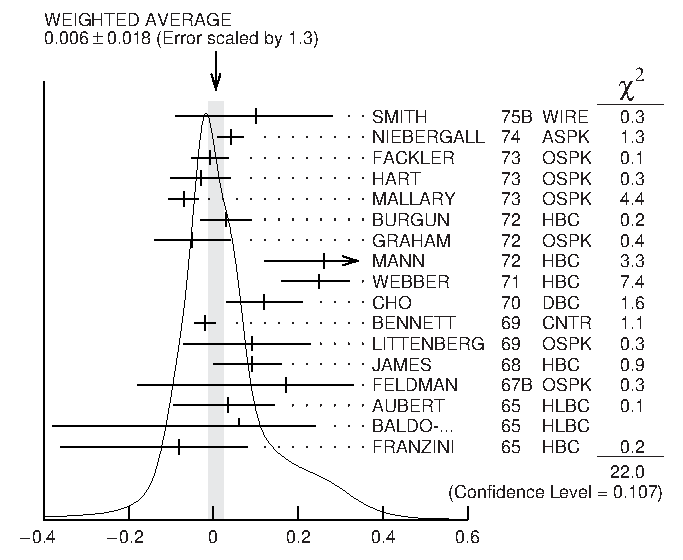
\includegraphics{filename.pdf}
	\caption{Example double wide figure, 
		with different book and web versions}
	\label{examples:fig:example2}
\end{pdgxfigure}
\end{verbtex}
\begin{pdgxfigure}[wide=true,place=h,width=0.45\textwidth] 
	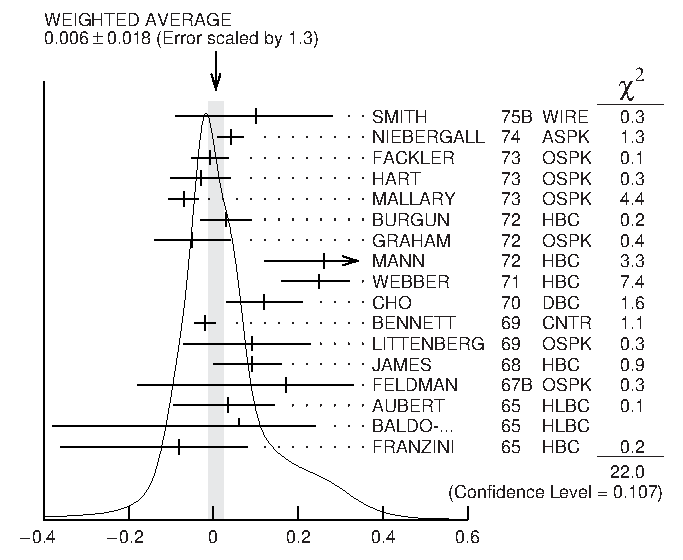
\includegraphics{filename.pdf}\hfill
	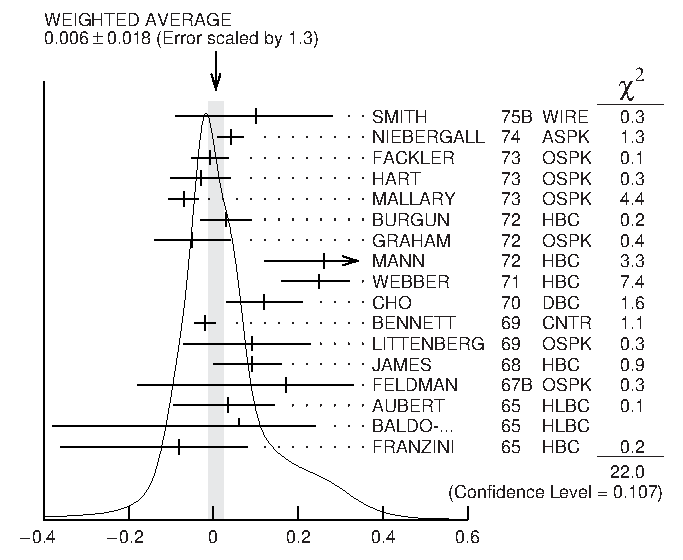
\includegraphics{filename.pdf}
	\caption{Example double wide figure, with different book and web versions}
	\label{examples:fig:example2}
\end{pdgxfigure}

A double wide figure with separate option and scaling keys, shown in Fig.~\ref{examples:fig:example3}:
\begin{verbtex}
\begin{pdgxfigure}[wide=true,place=h,width = 0.3\linewidth] 
	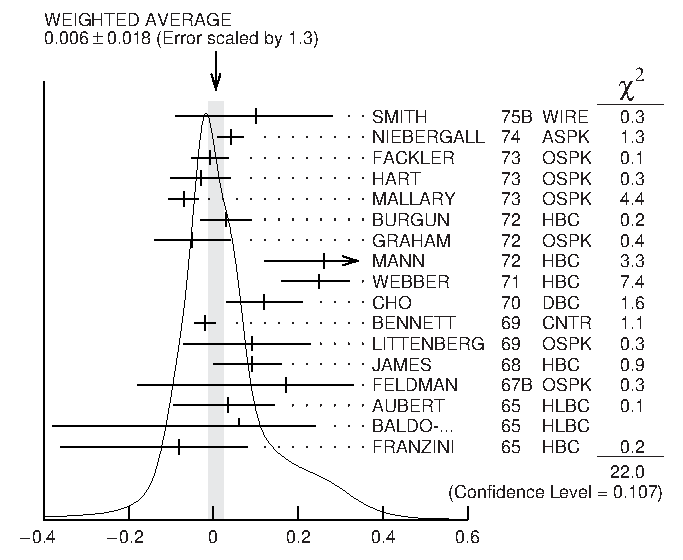
\includegraphics{filename.pdf}\hspace{1cm}
	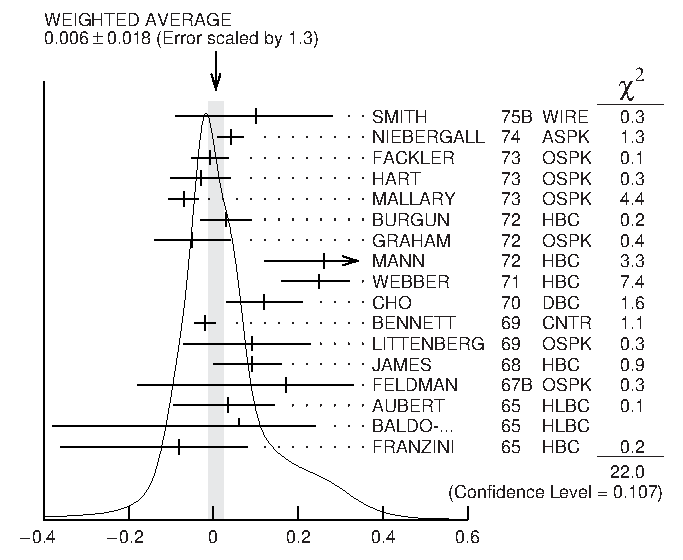
\includegraphics[width = !,scale =0.3,angle = 90]{filename}
	\caption{Example double figure, 
		with separate option and scaling keys, in both book and web versions}
	\label{examples:fig:example3}
\end{pdgxfigure}
\end{verbtex}
\begin{pdgxfigure}[wide=true,place=h,width = 0.3\linewidth] 
	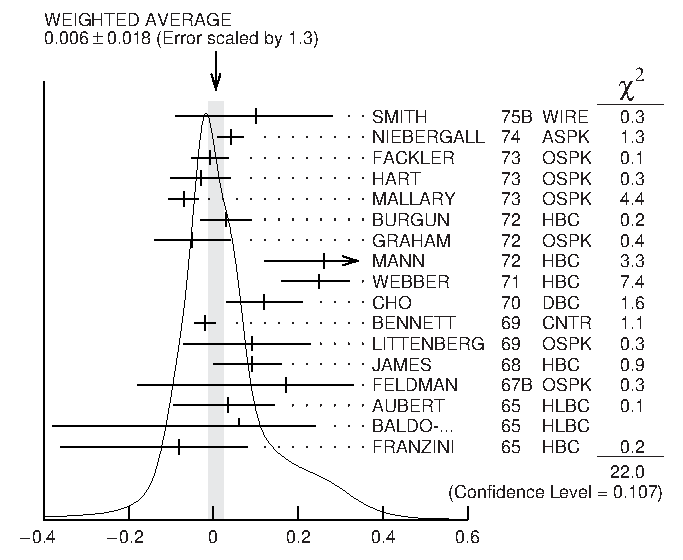
\includegraphics{filename.pdf}\hspace{1cm}
	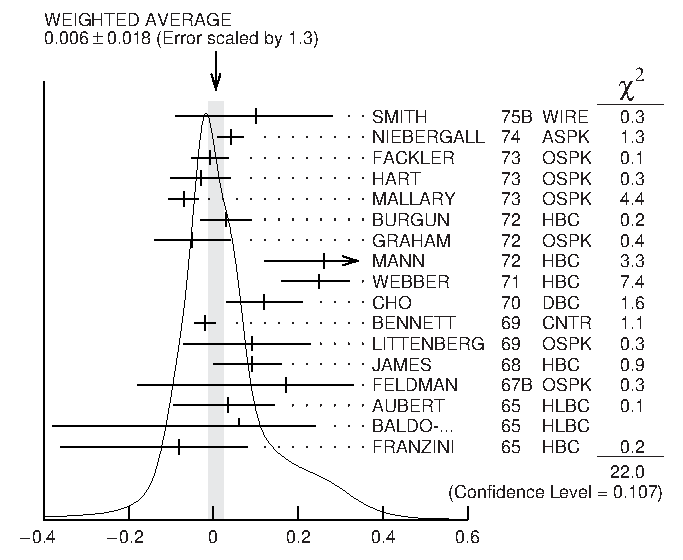
\includegraphics[width = !,scale =0.3,angle = 90]{filename}
	\caption{Example double wide figure, with separate option and scaling keys, in both book and web versions}
	\label{examples:fig:example3}
\end{pdgxfigure}

\Isubsection{\invt{pdgfigure} commands}
To add a figure, one may also use the \lstinline{\pdgfigure} or \lstinline{\pdgwidefigure} commands 
to typeset a single-column figure or double-column wide figure (for the book version), respectively. 
To include two images in one figure one may use \lstinline{\pdgdoublefigure}.
These commands are less powerful than \invt{pdgxfigure}, but automatically incorporate all PDG styles.

The macros \lstinline{\pdgfigure} and \lstinline{\pdgwidefigure} take the following arguments:
\begin{verbtex}
	\pdgfigure{<filename>}
	{<caption>}{<label>}{<placement options>}
	{<other option keys>}
\end{verbtex}
\vspace{-10pt}
while the macro \lstinline{\pdgdoublefigure} takes the following arguments:
\begin{verbtex}
	\pdgdoublefigure{<filename1>}{<filename2>}
	{<caption>}{<label>}{<placement options>}
	{<other option keys>}
\end{verbtex}
Some examples of the \invt{pdgfigure} commands are shown in Figs.~\ref{examples:fig:ideogram1}, \ref{examples:fig:ideogram2} and \ref{examples:fig:ideogram3}, respectively:
\begin{verbtex}
	\pdgfigure{filename.pdf}{Figure with caption and label}
	{examples:fig:ideogram1}{ht!}{}
	
	\pdgdoublefigure{filename.pdf}{filename.pdf}
	{Two figures, with caption and label, reduced in size}
	{examples:fig:ideogram2}{ht!}{width=0.3\textwidth}
	
	\pdgwidefigure{filename.pdf}{Wide figure}
	{examples:fig:ideogram3}{t}{}
\end{verbtex}
\FloatBarrier
\pdgfigure{filename.pdf}{Figure with caption and label}{examples:fig:ideogram1}{ht!}{}
\pdgdoublefigure{filename.pdf}{filename.pdf}{Two figures, with caption and label, reduced in size}{examples:fig:ideogram2}{ht!}{width=0.3\textwidth}
\pdgwidefigure{filename.pdf}{Wide figure}{examples:fig:ideogram3}{t}{}
\FloatBarrier

\Isection{Tables}
\label{sec:tables}
\Isubsection{ \invt{pdgxtable} and \invt{pdgxtabular}}
The PDG class provides multipurpose table and tabular environments, \invt{pdgxtable} and \invt{pdgxtabular}. 
These operate similarly to the standard \invt{table} and \invt{tabular} environments: \invt{(pdgx)table} creates a floating environment, 
while \invt{(pdgx)tabular} creates the actual tabulated display. 

The \lstinline!\caption! and \lstinline!\label! commands may be used as in the usual \invt{table} environment.
\textbf{Note: A table caption should be placed above the table.}
In addition, \invt{pdgxtable} takes a wide array of additional option keys that implement features and formatting of the prior PDG table commands/environments.  
These include keys that control placement, multicolumn spanning, version-specific widths and scaling (see Sec.~\ref{sec:ginkeys}), rotation, stretching, and caption widths.
The generic usage is
\begin{verbtex}
\begin{pdgxtable}[<option keys>]
	\caption{This is a PDG table}
	\label{tab:label}
	\begin{pdgxtabular}{<column settings>} % the usual c, l, r, | etc
		\pdgtableheader{...} %column header & separated entries go here
		%table & separated entries go here
	\end{pdgxtabular}
	%multiple pdgtabular environments are allowed
\end{pdgxtable}
\end{verbtex}

As for the usual \invt{table} environment, one may include multiple \invt{pdgxtabular}s in a single \invt{pdgxtable}.
While the \invt{pdgxtable} environment has default handling for caption widths in wide and regular tables, for both book and web versions, 
absolute control of the caption width can be implmented with a \lstinline{\captionsetup} command inside the \invt{pdgxtable} environment. 
For example \lstinline!\captionsetup{width=\linewidth}! gives a full width caption.

\Isubsection{Available keys for \invt{pdgxtable}}
Following is a list of available optional keys, and default settings if not invoked.
As usual, keys are evaluated left to right. 
While, the version-general \invt{width} key can be used (and will override any preceeding version-specfic width key), 
there is no version-general \invt{scale} key. 
Scaling of the tables is best done with the \invt{<version>scale} keys.

\begin{itemize}
	\item \invt{place}: Takes any combination of \invt{h}, \invt{t}, \invt{b}, \invt{p} (with optional \invt{\!}) that specifies float placement. Default is \invt{\!ht}.
	\item \invt{wide}: Takes \invt{true} or \invt{false} to specify the table as full page width in either single or two column mode. Default is \invt{false}.
	\item \invt{width} or \invt{<version>width}: Sets the version specific maximum width of the table bounding box. 
	Default is the maximum text width implied by the \invt{wide} key setting.
	Width settings exceeding this default are ineffective. Footnotes are scaled, but caption width is not affected.
	\item \invt{<version>scale}: Scales the table according to float value passed to the key. 
	For overwide tables, there is always a value $<1$ at which the table will be properly set to maximum page width.
	Footnotes are scaled, but caption width is not affected. Note the global \invt{scale} is disabled for \invt{pdgxtable}.
	\item \invt{<version>bbscale}: Scales the bounding box of the table. 
	For some overwide tables that are larger than the nominal page width, simply rescaling down the table does not allow the table to be properly aligned on the page.
	This key can be increased above $1$ (the default), to provide a sufficiently large bounding box for the table, that may then be scaled down to size with correct alignment.
	\item \invt{widecaptionscale}: For \invt{wide = true} tables, scales the caption width with respect to the maximum page width. Default is $0.75$.
	\item \invt{narrowcaptionscale}: For \invt{wide = false} or default tables, scales the caption width with respect to the maximum column width. Default is $0.9$.
	\item \invt{rotated}: Takes \invt{left} or \invt{right} to rotate the table, but not the caption, $90^\circ$ anticlockwise or clockwise, respectively. 
	The caption may be rotated independently, as needed with a \lstinline{\rotatebox}.
	\item \invt{sideways}: Takes \invt{true} or \invt{false} to rotate the table, including the caption, $90^\circ$ anticlockwise or clockwise, 
	according to whether the page number is even or odd.
	In a sideways table, other key width and scaling settings are still effective, but scale with respect to the page height. 
\end{itemize}


\Isubsection{Examples}
Some (simple) examples of \invt{pdgxtable} can be found in Table~\ref{examples:tab:styles} and Sec~\ref{sec:macros}.
For example, Tab.~\ref{examples:tab:styles} is typeset as
\begin{verbtex}
\begin{pdgxtable}[place=h,bookscale = 0.9,bookbbscale=2]
	\caption{Styles for the different typesetting versions}
	\label{examples:tab:styles}
	\begin{pdgxtabular}{ccccc}
		Version 		& Columns  & Font size 	& Helper Tags\footnote{
			Tags for each equation, table, figure, and bibliography entry 
			are displayed in margin or interspaced} & Line numbers\\
		\hline
		draft	& 1		   & 11pt		& Yes & Yes \\
		...
	\end{pdgxtabular}
\end{pdgxtable}
\end{verbtex}

Tables~\ref{examples:tab:commu} and~\ref{examples:tab:commp} are typeset as a two \invt{pdgxtabular}s in a single \invt{pdgxtable}, via
\begin{verbtex}
\begin{pdgxtable}[wide=true, place=!ht, webscale = 0.8]
	\caption{Common units}
	\label{examples:tab:commu}
	\begin{pdgxtabular}{lr | lr | lr}
		\showsymbol{\TeV} &  \showsymbol{\syin} & \showsymbol{\barn}   \\
		...
	\end{pdgxtabular}
	\caption{Common particles}
	\label{examples:tab:commp}
	\begin{pdgxtabular}{lr | lr | lr}
   		\showsymbol{\pp} &  \showsymbol{\ee} & \showsymbol{\pizero}   \\
  		...
	\end{pdgxtabular}
\end{pdgxtable}
\end{verbtex}

\Isubsection{Common problems and recommendations}
The \invt{pdgxtabular} environment is capable of handling the usual \lstinline{\multicolumn} and \lstinline{\multirow} objects, 
that allow for more complicated tables with cells spanning multiple rows and/or columns. 
We recommend avoiding use of \lstinline{\multispan}. 
For multiline cells, the \lstinline{\makecell} command from the \invt{makecell} package is recommended.

\Isection{Labels and referencing}
\label{sec:labels}

\Isubsection{Style guide}
As usual, the \lstinline{\label} and \lstinline{\ref} commands (and their derivatives) may be used to reference equations, tables, figures, and so on. 
To permit easy cross-referencing throughout the entire review, we request that you use the following labelling convention: \invt{BASENAME:type:name}
with \invt{type} corresponding to one of the following options
\begin{itemize}
\item {\tt fig} for figures
\item {\tt eq } for equation
\item {\tt tab} for tables
\item {\tt sec} for section, subsection etc..
\item {\tt foot} for footnotes.
\end{itemize}

\Isubsection{Missing references}

In default LaTeX, missing references are typically typeset as ``\textbf{??}''. 
To improve the typesetting experience, the \lstinline{\ref} command has been modified in the PDG class so that missing reference keys are printed out explicitly: 
For instance, a \lstinline!\ref{eqn:name}! that references a missing label called \invt{eqn:name}, will display as \ref{eqn:name}.
Similarly, the \lstinline{\cite} command will explicitly print out missing citation references. E.g. 
a \lstinline!\cite{name:2021ab}! that references a missing label called \invt{name:2021ab}, will display as \cite{name:2021ab}

\Isubsection{Cross-review referencing}
It is occasionally necessary or useful to reference (sub)sections, equations, figures, tables and so on belonging to other reviews or other reviews themselves. 
\textbf{Note:} Please use the \lstinline{\crossref} command for cross-review referencing.

Implementing a cross-reference to another review requires knowledge of its  \invt{BASENAME}:  
You must use the \invt{BASENAME} associated with the target review, not the \invt{BASENAME} of the review you're currently working on. 
To identify the  \invt{BASENAME} of another review, login into the \href{https://pdgworkspace.lbl.gov/Reviews.action}{PDG Workspace} (click to be redirected). 
Under \emph{Reviews} select from the drop-down menu \emph{All reviews}. 
Click on the title of the review you are interested in, and then select the \emph{Technical details} tab. 
The \invt{BASENAME} is the first entry.


If the full \invt{BASENAME:type:name} reference is known, you may include it with the usage \\
\lstinline!\crossref{BASENAME:type:name}!. 
This will typeset in your document as ``\crossref{BASENAME:type:name}'', because your local auxiliary files do not have the reference information of the other review.
PDG editorial staff will implement the cross-reference properly, when your review is prepared for production.

If the \invt{BASENAME:type:name} reference is not known, or the authors of the other review did not label the obect that you wish to reference, 
you may instead provide any descriptive argument to \lstinline{\crossref}. 
For example, \lstinline!\crossref{Equation 34.1.10}!.  
PDG editorial staff will implement the cross-reference properly, when your review and the other review are prepared for production.

\Isubsection{Booklet labeling and referencing}
If your review has a booklet version, it needs to be prepared at the same time as you prepare your full review.
The content to be displayed in the booklet needs to be included in \invt{BASENAME-booklet.tex}. 

The numerical tags for equations, tables, and figures in the booklet version of a review should match the tags in the full version. 
This can be achieved automatically in the booklet version by using a \lstinline!\tag{\ref{BASENAME:type:name}}! construction instead of \lstinline{\label}
to refer to the reference in the full version.
For example, if the full version has a labelled equation
\begin{verbtex}
\begin{equation}
	\label{BASENAME:eq:name}
	...
\end{equation}
\end{verbtex}
then including in \invt{BASENAME-booklet.tex}
\begin{verbtex}
\begin{equation}
	\tag{\ref{BASENAME:eq:name}}
	...
\end{equation}
\end{verbtex}
will automatically label the equation correctly. 
To achieve the same result for figures and tables, one may place in the booklet version
\begin{verbtex}
	\renewcommand{\thetable}{\ref{BASENAME:type:name}}
	\renewcommand{\thefigure}{\ref{BASENAME:type:name}}
\end{verbtex}
before each table or figure environment, respectively. 


\Isection{Index entries}
\label{sec:index}

Review authors should think about any keywords that should be included into the index of the Review of Particle Physics. PDG uses the standard \LaTeX\  \invt{makeidx} package. Thus an entry ``sample text'' can be added to the index by placing
\begin{verbtex}
\index{sample text}
\end{verbtex}
at the appropriate place in the source file. Formatting of entries with Greek letters or math symbols as well as subentries are also supported. For example
\begin{verbtex}
\index{sigma@$\$$\sigma$\$$} 
\end{verbtex}
creates an index entry $\sigma$ in the proper alphabetical order, while
\begin{verbtex}
\index{Searches!Axion searches} 
\end{verbtex}
produces a subentry ``Axion searches'' under the ``Searches'' index entry.

All index entries defined in a given review will be shown on the last page when the draft version is made. PDG staff will standardize all index entries during the final processing of all reviews. Therefore what matters is not the final formatting of index entries but that all relevant entries are added in the correct place.


\Isection{Bibliography}
\label{sec:cites}

Citations are handled using BibTeX. To add a citation to your review:
\begin{itemize}
\item Look up the reference in INSPIRE and download its BibTeX entry (see bottom of the \emph{Information} tab for the article, under \emph{Export}).
\item Add the BibTeX entry to the \invt{BASENAME.bib} file. Note the article tag assigned by INSPIRE: You can see it in the first line of the BibTeX entry, after \lstinline!@article{!.
\item Cite the reference with \lstinline{\cite}, using the article tag assigned by INSPIRE.
\end{itemize}

For example, to add a reference to the Review of Particle Physics (2018) 
add the following code to \invt{BASENAME.bib}:
\begin{verbtex}
@article{Tanabashi:2018oca,
      author         = "Tanabashi, M. and others",
      title          = "{Review of Particle Physics}",
      collaboration  = "Particle Data Group",
      journal        = "Phys. Rev.",
      volume         = "D98",
      year           = "2018",
      number         = "3",
      pages          = "030001",
      doi            = "10.1103/PhysRevD.98.030001",
      SLACcitation   = "%%CITATION = PHRVA,D98,030001;%%"
 }
\end{verbtex}
and then one may add a reference to it in \invt{BASENAME-main.tex} via \lstinline!\cite{Tanabashi:2018oca}!.

If a BibTeX entry downloaded from INSPIRE does not render correctly, 
you should first make sure you have the latest PDG style files, by running \invt{svn update} (after committing any edits you have made).
If this doesn't fix the issue please contact \invt{latexsupport@pdg.lbl.gov} for advice.  
If it appears, however, to be simply a mistake in INSPIRE's entry, 
rename the label to the form \invt{BASENAME:<INSPIRE label>} and then edit the entry as needed.
\textbf{Please do not edit entries downloaded from INSPIRE without changing the label.}
Changing the label will permit PDG editorial staff to easily identify and track edited citations, as well as notify INSPIRE of required corrections.
In case the reference does not appear in INSPIRE at all, please also use the convention for the label: \invt{BASENAME:name}.

Multiple references can be added to a single set of brackets with \lstinline!\cite{cite-key-1,cite-key-2,...}!.
One may group multiple references into the same numerical citation tag, using a \invt{*} prefix on subsequent citation keys: For example \lstinline!\cite{cite-key-1,*cite-key-2,*cite-key-3}!.
If a paper citation key is preceded by the asterisk, it can't be cited separately later, and doing so will result in a compilation error.
We recommend citing papers individually, without using the asterisk to group them.


\Isection{Footnotes}
Footnote styles are standardized throughout the review. In (rare) cases that the style needs to be changed, this is achieved via \lstinline!\setfootnotestyle{<style>}!,
where \invt{<style>} can be \lstinline{\fnsymbol} or \lstinline{\alph}, \lstinline{\Alph}, \lstinline{\arabic}, \lstinline{\roman}, \lstinline{\Roman} etc.

Sometimes the \LaTeX \ engine miscalculates the amount of space required for a footnote, resulting in overprinting of the footer.
One can help the engine obtain a better estimate by adjusting the effective page size. 
This can be done by placing \lstinline!\enlargethispage{-2\baselineskip}! somewhere just before the \lstinline{\footnote}; the \invt{-2} may be changed to any number. 

\Isection{Miscellaneous control commands}

\Isubsection{Unbalanced last page}
In the book version, the columns of the final page are automatically balanced. 
If this behavior is undesired, it may be altered by invoking \lstinline!\balancedlastpagefalse!.
The invocation may be added anywhere in the document.

\Isubsection{Blank last page}
In the book version, a blank final page may be added via \lstinline!\blankendpagetrue!.
The invocation may be added anywhere in the document.

\Isubsection{Book-only reviews}
Certain reviews are typeset for the web using the book version formatting. 
This is enforced automatically within the PDG system by \lstinline!\def\iswebbook{1}! before the \lstinline{\documentclass} invocation. 
The draft version, however, for such reviews are typeset in the usual draft/web format.

\clearpage
\Isection{PDG Macros}
\label{sec:macros}

\begin{pdgxtable}[wide=true, place=!ht, webscale = 0.8]
	\vspace{-10pt}
	\caption{Common units}
	\label{examples:tab:commu}
	\begin{pdgxtabular}{lr | lr | lr}
		\showsymbol{\TeV     } &  \showsymbol{\syin} & \showsymbol{\barn     }   \\
		\showsymbol{\MeV     } &  \showsymbol{\inch} & \showsymbol{\mbarn    }   \\
		\showsymbol{\keV     } &  \showsymbol{\ft  } & \showsymbol{\microbarn}   \\
		\showsymbol{\eV      } &  \showsymbol{\km  } & \showsymbol{\nb       }   \\
		\showsymbol{\GeVc    } &  \showsymbol{\m   } & \showsymbol{\pb       }   \\
		\showsymbol{\GeVcSq  } &  \showsymbol{\cm  } & \showsymbol{\fb       }   \\
		\showsymbol{\GeVcc   } &  \showsymbol{\mm  } & \showsymbol{\invnb    }   \\
		\showsymbol{\GeVccSq } &  \showsymbol{\mum } & \showsymbol{\invpb    }   \\
		\showsymbol{\MeVc    } &  \showsymbol{\nm  } & \showsymbol{\invfb    }   \\
		\showsymbol{\MeVcc   } &  \showsymbol{\fm  } & \showsymbol{\invab    }   \\
		\showsymbol{\invps   } &  \showsymbol{\nm  } & \showsymbol{\lum      }   \\
			&&  \showsymbol{\ma  } &&  \\
		\showsymbol{\degr    }  &  \showsymbol{\cma } && \\
			&&  \showsymbol{\mma } &&   \\
			&&  \showsymbol{\muma} &&   \\
	\end{pdgxtabular}
	\vspace{10pt}
	\caption{Common particles}
	\label{examples:tab:commp}
	\vspace{-10pt}
	\begin{pdgxtabular}{lr | lr | lr}
   \showsymbol{\pp         } &  \showsymbol{\ee           } & \showsymbol{\pizero   }   \\
   \showsymbol{\pbar       } &  \showsymbol{\epm          } & \showsymbol{\piplus   }   \\
   \showsymbol{\ppbar      } &  \showsymbol{\epem         } & \showsymbol{\piminus  }   \\
   \showsymbol{\tbar       } &  \showsymbol{\en           } & \showsymbol{\pipm     }   \\
   \showsymbol{\ttbar      } &  \showsymbol{\ep           } & \showsymbol{\pimp     }   \\
   \showsymbol{\bbar       } &  \showsymbol{\mumu         } & \showsymbol{\etaprime }   \\
   \showsymbol{\bbbar      } &  \showsymbol{\mun          } & \showsymbol{\Kzero    }   \\
   \showsymbol{\cbar       } &  \showsymbol{\mup          } & \showsymbol{\Kzerobar }   \\
   \showsymbol{\ccbar      } &  \showsymbol{\tautau       } & \showsymbol{\kaon     }   \\
   \showsymbol{\sbar       } &  \showsymbol{\taup         } & \showsymbol{\Kplus    }   \\
   \showsymbol{\ssbar      } &  \showsymbol{\taum         } & \showsymbol{\Kminus   }   \\
   \showsymbol{\ubar       } &  \showsymbol{\lepton       } & \showsymbol{\KzeroL   }   \\
   \showsymbol{\uubar      } &  \showsymbol{\leptonm      } & \showsymbol{\Kzerol   }   \\
   \showsymbol{\dbar       } &  \showsymbol{\ellm         } & \showsymbol{\Klong    }   \\
   \showsymbol{\ddbar      } &  \showsymbol{\leptonp      } & \showsymbol{\KzeroS   }   \\
   \showsymbol{\fbar       } &  \showsymbol{\ellp         } & \showsymbol{\Kzeros   }   \\
   \showsymbol{\ffbar      } &  \showsymbol{\leptonlepton } & \showsymbol{\Kshort   }   \\
   \showsymbol{\qbar       } &  \showsymbol{\ellell       } & \showsymbol{\Kstar    }   \\
   \showsymbol{\qqbar      } &  \showsymbol{\enu          } & \showsymbol{\jpsi     }   \\
   \showsymbol{\nbar       } &  \showsymbol{\munu         } & \showsymbol{\Jpsi     }   \\
   \showsymbol{\nnbar      } &  \showsymbol{\taunu        } & \showsymbol{\psip     }   \\
   \showsymbol{\neutron    } &  \showsymbol{\lnu          } & \showsymbol{\chic     }   \\
   \showsymbol{\antineutron} &  \showsymbol{\nub          } & \showsymbol{\UoneS    }   \\
   \showsymbol{\deuteron   } &  \showsymbol{\nunub        } & \showsymbol{\chib     }   \\
   \showsymbol{\Zzero      } &  \showsymbol{\nue          } & \showsymbol{\Dstar    }   \\
   \showsymbol{\Zboson     } &  \showsymbol{\nueb         } & \showsymbol{\Bd       }   \\
   \showsymbol{\Wplus      } &  \showsymbol{\nuenueb      } & \showsymbol{\Bs       }   \\
   \showsymbol{\Wminus	   } &  \showsymbol{\num          } & \showsymbol{\Bu       }   \\
   \showsymbol{\Wboson	   } &  \showsymbol{\numb         } & \showsymbol{\Bc       }   \\ 
   \showsymbol{\Wpm   	   } &  \showsymbol{\numnumb      } & \showsymbol{\Lb       }   \\
   \showsymbol{\Wmp        } &  \showsymbol{\nut          } & \showsymbol{\Bstar    }   \\
   \showsymbol{\Hzero } &  \showsymbol{\nutb         } & \showsymbol{\BoBo     }   \\
   \showsymbol{\Hboson}  &	\showsymbol{\nutnutb      } & \showsymbol{\BodBod   }    \\		    
   \showsymbol{            } &	\showsymbol{              } & \showsymbol{\BosBos   }    \\		    
   \showsymbol{            } &	\showsymbol{              } & \showsymbol{\LambdaStar}  \\
	\end{pdgxtabular}
\end{pdgxtable}

\begin{pdgxtable}[wide=true, place=h, webscale = 0.8]
	\caption{Hypothetical particles}
	\begin{pdgxtabular}{lr | lr | lr}
   \showsymbol{\Azero }      &  \showsymbol{\gravino   } & \showsymbol{\slepton   }   \\
   \showsymbol{\hzero }      &  \showsymbol{\Zprime    } & \showsymbol{\sleptonL  }   \\
   \showsymbol{\Hzero }      &  \showsymbol{\Zstar     } & \showsymbol{\sleptonR  }   \\
   \showsymbol{\Hplus }  	  &  \showsymbol{\squark    } & \showsymbol{\sel       }   \\
   \showsymbol{\Hminus}       &  \showsymbol{\squarkL   } & \showsymbol{\selL      }   \\
   \showsymbol{\Hpm   }   	&  \showsymbol{\squarkR   } & \showsymbol{\selR      }   \\
   \showsymbol{\Hmp   }       &  \showsymbol{\gluino    } & \showsymbol{\smu       }   \\
   \showsymbol{\ggino }     &  \showsymbol{\stop      } & \showsymbol{\smuL      }   \\
   \showsymbol{\chinop}      &  \showsymbol{\stopone   } & \showsymbol{\smuR      }   \\
   \showsymbol{\chinom}      &  \showsymbol{\stoptwo   } & \showsymbol{\stau      }   \\
   \showsymbol{\chinopm}      &  \showsymbol{\stopL     } & \showsymbol{\stauL     }   \\
   \showsymbol{\chinomp}     &  \showsymbol{\stopR     } & \showsymbol{\stauR     }   \\
   \showsymbol{\chinoonep}     &  \showsymbol{\sbottom   } & \showsymbol{\stauone   }   \\
   \showsymbol{\chinoonem}   &  \showsymbol{\sbottomone} & \showsymbol{\stautwo   }   \\
   \showsymbol{\chinoonepm}   &  \showsymbol{\sbottomtwo} & \showsymbol{\snu       }   \\
   \showsymbol{\chinotwop}  &  \showsymbol{\sbottomL  } & \showsymbol{           }   \\
   \showsymbol{\chinotwom}   &  \showsymbol{\sbottomR  } & \showsymbol{           }   \\
   \showsymbol{\chinotwopm}   &  \showsymbol{           } & \showsymbol{           }   \\
   \showsymbol{\nino}  &  \showsymbol{           } & \showsymbol{           }   \\
   \showsymbol{\ninoone}        &  \showsymbol{           } & \showsymbol{           }   \\
   \showsymbol{\ninotwo}     &  \showsymbol{           } & \showsymbol{           }   \\
   \showsymbol{\ninothree}     &  \showsymbol{           } & \showsymbol{           }   \\
   \showsymbol{\ninofour}   &  \showsymbol{           } & \showsymbol{           }   \\
	\end{pdgxtabular}
\vspace*{10pt}
	\caption{Useful symbols for proton-proton physics}
\vspace*{-10pt}	
	\begin{pdgxtabular}{lr | lr }
   \showsymbol{\pT  }      &  \showsymbol{\rts }   \\
   \showsymbol{\pt  }      &  \showsymbol{\sqs } \\
   \showsymbol{\ET  }      &  \showsymbol{\mh}  \\
   \showsymbol{\eT  }      &  \showsymbol{\mW}  \\
   \showsymbol{\et  }      & \showsymbol{\mZ}   \\
   \showsymbol{\HT  }      & \showsymbol{\mH}   \\
   \showsymbol{\pTsq}      &&   \\
   \showsymbol{\MET }      &&   \\
   \showsymbol{\met }      &&   \\
   \showsymbol{\Ecm }      &&   \\
	\end{pdgxtabular}
\vspace*{10pt}
	\caption{Monte Carlo Generators}
\vspace*{-10pt}		
	\begin{pdgxtabular}{lr | lr | lr}	
   \showsymbol{\ACERMC    }      &  \showsymbol{\MCatNLO   } & \showsymbol{\Comphep    }   \\
   \showsymbol{\ALPGEN    }      &  \showsymbol{\AMCatNLO  } & \showsymbol{\Prospino   }   \\
   \showsymbol{\GEANT     }      &  \showsymbol{\MCFM      } & \showsymbol{\LO         }   \\
   \showsymbol{\Herwigpp  }      &  \showsymbol{\METOP     } & \showsymbol{\NLO        }   \\
   \showsymbol{\HERWIGpp  }      &  \showsymbol{\POWHEG    } & \showsymbol{\NLL        }   \\
   \showsymbol{\Herwig    }      &  \showsymbol{\POWHEGBOX } & \showsymbol{\NNLO       }   \\
   \showsymbol{\HERWIG    }      &  \showsymbol{\POWPYTHIA } & \showsymbol{\muF        }   \\
   \showsymbol{\JIMMY     }      &  \showsymbol{\PROTOS    } & \showsymbol{\muR        }   \\
   \showsymbol{\MADSPIN   }      &  \showsymbol{\PYTHIA    } & \showsymbol{            }   \\
   \showsymbol{\MADGRAPH  }      &  \showsymbol{\SHERPA    } & \showsymbol{            }   \\
   \showsymbol{\MGMCatNLO }      &  \showsymbol{           } & \showsymbol{            }   \\
	\end{pdgxtabular}
\end{pdgxtable}

\Isection{Tables: Legacy commands}

Though no longer recommended, legacy \lstinline{\pdgtable} or \lstinline{\pdgwidetable} commands 
to typeset a single-column table or double-column wide table (for the book version), respectively.
The \lstinline{\pdgtableheader} macro may be used in the first line of the table to automatically typeset a header.

The macros \lstinline{\pdgtable} and \lstinline{\pdgwidetable} take the following arguments:
\begin{verbtex}
	\pdgtable{<column styles>}
	{<caption>}{<label>}{<option keys>}
\end{verbtex}
Some examples usages of these commands follow, in Tables~\ref{examples:tab:table1}, \ref{examples:tab:table2} and~\ref{examples:tab:table3} below.
\begin{verbtex}
\begin{pdgtable}{c c c} 
	{Table}{examples:tab:table1}{h!}
	\pdgtableheader{ Column 1 & Column 2 & Column 3}
	row1  & 1  & 2\\
	row2  & 1  & 2\\
	row3  & 1  & 2\\
\end{pdgtable}
\end{verbtex}   
\begin{verbtex}
\begin{pdgtable}{|c | c | c | c|} 
	{Multicolumn table}{examples:tab:table2}{h!}
	\pdgtableheader{ \multicolumn{2}{c}{Column 1} & 
	\multicolumn{2}{c}{Column 2}}
	\pdgtableheader{ A & B& C & D }
	row1  & 1 & 2 &3 \\
	row2  & 1 & 2 &3 \\
\end{pdgtable}
\end{verbtex}  
\begin{verbtex}
\begin{pdgtable}{c l}
	{Table with footnotes}{examples:tab:table3}{}
	One value & another\footnote{This is something to notice
	\label{kmmix:foot:one}}\\
	Two values\footref{kmmix:foot:one} & another \\
\end{pdgtable}
\end{verbtex} 
 
\FloatBarrier 
\begin{pdgtable}{c c c} 
{Table}{examples:tab:table1}{h!}
\pdgtableheader{ Column 1 & Column 2 & Column 3}
row1  & 1  & 2\\
row2  & 1  & 2\\
row3  & 1  & 2\\
\end{pdgtable}
\begin{pdgtable}{|c | c | c | c|} 
{Multicolumn table}{examples:tab:table2}{h!}
\pdgtableheader{ \multicolumn{2}{|c|}{Column 1} & 
\multicolumn{2}{|c|}{Column 2}}
\pdgtableheader{ A & B& C & D }
row1  & 1 & 2 &3 \\
row2  & 1 & 2 &3 \\
\end{pdgtable}
\begin{pdgtable}{c l}
{Table with footnotes}{examples:tab:table3}{}
One value & another\footnote{This is something to notice\label{kmmix:foot:one}}\\
Two values\footref{kmmix:foot:one} & another \\
\end{pdgtable}

\section{Introduction}\label{introduction}

The collection of online information resources in particle physics and
related areas presented in this chapter is of necessity incomplete. An
expanded and regularly updated online version can be found at:
\url{http://library.cern/particle_physics_information}

Suggestions for additions and updates are very welcome.\footnote{Please
  send comments and corrections to micha.moshe.moskovic@cern.ch}

\section{Particle Data Group (PDG)
resources}\label{particle-data-group-pdg-resources}

\begin{itemize}
\item
  \textbf{Review of Particle Physics (RPP):} A comprehensive report on
  the fields of particle physics and related areas of cosmology and
  astrophysics, including both review articles and a
  compilation/evaluation of data on particle properties. The review
  section includes articles, tables and plots on a wide variety of
  theoretical and experimental topics of interest to particle physicists
  and astrophysicists. The particle properties section provides tables
  of published measurements as well as the Particle Data Group's best
  values and limits for particle properties such as masses, widths,
  lifetimes, and branching fractions, as well as an extensive summary of
  searches for hypothetical particles. RPP is published as a large book
  every two years, with partial updates made available once each year on
  the web.

  All the contents of the book version of RPP are available online:
  \url{http://pdg.lbl.gov}

  The printed book can be ordered:
  \url{http://pdg.lbl.gov/2019/html/receive_our_products.html}

  Of historical interest is the complete RPP collection which can be
  found online: \url{http://pdg.lbl.gov/rpp-archive/}
  \url{http://library.cern/PDG_publications/review_particle_physics}
\item
  \textbf{Particle Physics booklet:} An abridged version of the Review
  of Particle Physics, available as a pocket-sized 250-page booklet. It
  is one of the most useful summaries of physics data. The booklet
  contains an abbreviated set of reviews and the summary tables from the
  most recent edition of the Review of Particle Physics.

  The PDF file of the booklet can be downloaded:
  \url{http://pdg.lbl.gov/current/booklet.pdf}

  The printed booklet can be ordered:
  \url{http://pdg.lbl.gov/2019/html/receive_our_products.html}
\item
  \textbf{PDGLive:} A web application for browsing the contents of the
  PDG database that contains the information published in the Review of
  Particle Physics. It allows one to navigate to a particle of interest,
  see a summary of the information available, and then proceed to the
  detailed information published in the Review of Particle Physics. Data
  entries are directly linked to the corresponding bibliographic
  information in INSPIRE. \url{http://pdglive.lbl.gov}
\item
  \textbf{Computer-readable files:} Data files that can be downloaded
  from the PDG include tables of particle masses and widths, PDG Monte
  Carlo particle numbers, and cross-section data. The files are updated
  with each new edition of the Review of Particle Physics.
  \url{http://pdg.lbl.gov/current/html/computer_read.html}
\end{itemize}

\section{Particle Physics Information
Platforms}\label{particle-physics-information-platforms}

\begin{itemize}
\item
  \textbf{INSPIRE:} INSPIRE serves as a one-stop information platform
  for the particle physics community, comprising 8 interlinked databases
  on literature, conferences, institutions, journals, researchers,
  experiments, jobs and data. Run in collaboration by CERN, DESY,
  Fermilab, IHEP, IN2P3, and SLAC, it has been serving the scientific
  community for almost 50 years. Previously known as SPIRES, it was the
  first website outside Europe and the first database on the web. Close
  interaction with the user community and with arXiv, ADS, HEPData,
  ORCID, PDG and publishers is the backbone of INSPIRE's evolution.
  \url{http://inspirehep.net/}

  In 2019, INSPIRE launched INSPIRE beta, featuring all-new literature
  search, author profiles and job postings. INSPIRE beta is running in
  parallel with the current platform and it will fully replace it in the
  future. The INSPIRE beta site is available at:
  \url{http://beta.inspirehep.net}

  \begin{itemize}
  \tightlist
  \item
    Blog:
    \href{http://blog.inspirehep.net/}{\texttt{http://blog.inspirehep.net/}}
  \item
    Twitter: \href{https://twitter.com/inspirehep}{\texttt{@inspirehep}}
  \end{itemize}
\end{itemize}

\section{Literature Databases}\label{literature-databases}

\begin{itemize}
\item
  \textbf{ADS:} The SAO/NASA Astrophysics Data System is a Digital
  Library portal offering access to 13 million bibliographic records in
  Astronomy and Physics. The ADS search engine also indexes the
  full-text for approximately four million publications in this
  collection and tracks citations, which now amount to over 80 million
  links. The system also provides access and links to a wealth of
  external resources, including electronic articles hosted by publishers
  and arXiv, data catalogs and a variety of data products hosted by the
  astronomy archives worldwide. The ADS can be accessed at:
  \url{http://ads.harvard.edu/}
\item
  \textbf{arXiv.org:} A repository of full-text articles in physics,
  astronomy, mathematics, computer science, statistics, nonlinear
  sciences, quantitative finance, quantitative biology, electrical
  engineering and systems science, and economics. Papers are submitted
  by registered authors to arXiv, often as preprints in advance of
  submission to a journal for publication; includes postprints, working
  papers, and other relevant material. Established in 1991, the
  repository is interlinked with ADS and INSPIRE, among others. Readers
  can browse subject categories or search by author, title, abstract,
  date, and other fields. Receive daily update alerts for subfields by
  email or RSS. \url{https://arXiv.org}

  \begin{itemize}
  \tightlist
  \item
    Blog:
    \href{https://blogs.cornell.edu/arXiv}{\texttt{https://blogs.cornell.edu/arXiv}}
  \item
    Twitter: \href{https://twitter.com/arxiv}{\texttt{@arxiv}}
  \end{itemize}
\item
  \textbf{CDS:} The CERN Document Server contains records of about
  700,000 CERN and non-CERN articles, preprints, theses. It includes
  records for internal and technical notes, official CERN committee
  documents, and multimedia objects. CDS is planning to focus on its
  role as an institutional repository covering all CERN material from
  the early 50s and reflecting the holdings of the CERN library.
  Non-CERN particle and accelerator physics content is in the process of
  being exported to INSPIRE. \url{http://cds.cern.ch}
\item
  \textbf{INSPIRE HEP:} The HEP collection, the flagship of the INSPIRE
  suite, serves more than 1.3 million bibliographic records with a
  growing number of full-text articles attached and metadata including
  author affiliations, abstracts, references, experiments, keywords as
  well as links to arXiv, ADS, PDG, HEPData, publisher platforms and
  other servers. It provides fast metadata and full-text searches, plots
  extracted from full text, author disambiguation, author profile pages
  and citation analysis and is expanding its content to, e.g.,
  experimental notes. \url{http://inspirehep.net}
\item
  \textbf{JACoW:} The Joint Accelerator Conference Website publishes the
  proceedings of several accelerator conferences held around the world.
  A custom interface allows searching based on keywords, titles,
  authors, and in the full text. \url{http://www.jacow.org/}
\item
  \textbf{KEK Library Preprints and Reports Database:} This database
  contains bibliographic records of preprints and technical reports held
  in the KEK library, with links to the full-text images of more than
  100,000 papers scanned from their worldwide preprint collection.
  Particularly useful for older scanned preprints. Links to it are
  included in INSPIRE HEP.
  \url{https://www.i-repository.net/il/meta_pub/engG0000128Lib}
\item
  \textbf{MathSciNet:} This database of almost 3 million items provides
  reviews, abstracts and bibliographic information for much of the
  mathematical sciences literature. Over 100,000 new items, most of them
  classified according to the Mathematics Subject Classification, and
  more than 80,000 reviews of the current published literature are added
  each year. Author identification allows users to search for
  publications by author and citation data allows users to track the
  history and influence of research publications.
  \url{http://www.ams.org/mathscinet}
\item
  \textbf{OSTI.GOV:} A portal to free, publicly available DOE-sponsored
  R\&D results including technical reports, bibliographic citations,
  journal articles, conference papers, books, multimedia and data
  information. It consolidates OSTI's home page and the now-retired
  primary search tool SciTech Connect. It contains over 3 million
  records, including citations to 1.5 million journal articles, 1
  million of which have digital object identifiers (DOIs) linking to
  full-text articles on publishers' websites. \url{https://www.osti.gov}
\end{itemize}

\section{Particle Physics Journals and Conference Proceedings
Series}\label{particle-physics-journals-and-conference-proceedings-series}

\begin{itemize}
\item
  \textbf{CERN Journal List:} This list of journals and conference
  series publishing particle physics content provides information on
  Open Access, copyright policies and terms of use.
  \url{http://library.cern/oa/where-publish}
\item
  \textbf{INSPIRE Journals:} The database contains over 3,600 journals
  publishing HEP-related articles.
  \url{http://inspirehep.net/collection/journals}
\end{itemize}

\section{Conference Databases}\label{conference-databases}

\begin{itemize}
\tightlist
\item
  \textbf{INSPIRE Conferences:} The database of more than 23,000 past,
  present, and future conferences, schools, and meetings relevant to
  high-energy physics and related fields is searchable by title,
  acronym, series, date and location. Included are information about
  published proceedings, links to conference contributions in the
  INSPIRE HEP database, and links to the conference website when
  available. New conferences can be submitted from the entry page.
  \url{http://inspirehep.net/conferences}
\end{itemize}

\section{Research Institutions}\label{research-institutions}

\begin{itemize}
\tightlist
\item
  \textbf{INSPIRE Institutions:} INSPIRE Institutions contains over
  11,500 institutes, laboratories, and universities, where research on
  particle physics and astrophysics is led. Every record includes,
  whenever possible, as detailed information, such as address, web
  links, experiments, and links to INSPIRE papers authored by people
  affiliated to that institution. One can search for a particular
  institution by name, acronym, and location.
  \url{http://inspirehep.net/institutions}
\end{itemize}

\section{People}\label{people}

\begin{itemize}
\item
  \textbf{INSPIRE HEPNames:} Searchable worldwide database of over
  125,000 active, departed, retired, and deceased people associated with
  particle physics and related fields. The affiliation history of these
  researchers, their e-mail addresses, ORCIDs, web pages, experiments
  they participated in, PhD advisor, information on their graduate
  students and links to their papers in the INSPIRE HEP, arXiv and ADS
  databases are provided, as well as a user interface to update this
  information. \url{http://inspirehep.net/hepnames}
\item
  \textbf{ORCID}: Registry providing persistent digital identifiers
  allowing to unambiguously identify researchers. Through integration in
  key research workflows such as manuscript and grant submission, it
  supports automated linkages between scientists and their professional
  activities ensuring that their work is recognized.
  \url{https://orcid.org}
\end{itemize}

\section{Experiments}\label{experiments}

\begin{itemize}
\item
  \textbf{INSPIRE Experiments:} Contains more than 3,500 past, present,
  and future experiments in particle physics. Lists both accelerator and
  non-accelerator experiments. Includes official experiment name and
  number, location, and collaboration lists. Simple searches by
  participant, title, experiment number, institution, date approved,
  accelerator, or detector, return a description of the experiment,
  including a complete list of authors, title, overview of the
  experiment's goals and methods, and a link to the experiment's web
  page if available. Recently, it has expanded its scope to include
  particle accelerators besides experiments and to link them together.
  \url{http://inspirehep.net/Experiments}
\item
  \textbf{Cosmic ray/Gamma ray/Neutrino and similar experiments:} This
  extensive collection of experiment websites is organized by focus of
  study and by location. Additional sections link to educational
  materials, organizations, and other useful resources. The site is
  maintained at the Max Planck Institute for Nuclear Physics,
  Heidelberg.
  \url{http://www.mpi-hd.mpg.de/hfm/CosmicRay/CosmicRaySites.html}
\end{itemize}

\section{Jobs}\label{jobs}

\begin{itemize}
\item
  \textbf{AAS Job Register:} The American Astronomical Society publishes
  once a month graduate, postgraduate, faculty and other positions
  mainly in astronomy and astrophysics.
  \url{http://jobregister.aas.org/}
\item
  \textbf{Academic Jobs Online}: A full-service online recruiting site
  for academic institutions worldwide in all disciplines and areas.
  \url{https://academicjobsonline.org/ajo}
\item
  \textbf{APS Careers:} A gateway for physicists, students, and physics
  enthusiasts to information about physics jobs and careers. It contains
  Physics job listings, career advice, upcoming workshops and meetings,
  and career and job-related resources provided by the American Physical
  Society. \url{http://www.aps.org/careers/employment}
\item
  \textbf{brightrecruits.com:} A recruitment service run by IOP
  Publishing that connects employers from different industry sectors
  with jobseekers who have a background in physics and engineering.
  \url{http://brightrecruits.com/}
\item
  \textbf{IOP Careers:} Career information and resources primarily aimed
  at university students are provided by the UK Institute of Physics.
  \url{http://www.iop.org/careers/}
\item
  \textbf{INSPIRE HEPJobs:} Lists academic and research jobs in high
  energy physics, nuclear physics, accelerator physics and astrophysics
  with the option to post a job or to receive email notices of new job
  listings. About 500 jobs are currently listed.
  \url{http://inspirehep.net/jobs}
\item
  \textbf{Physics Today Jobs:} Online recruitment advertising website
  for Physics Today magazine, published by the American Institute of
  Physics. Physics Today Jobs is the managing partner of the AIP Career
  Network, an online job board network for the physical science,
  engineering, and computing disciplines. Over 6,000 resumes are
  currently available, and nearly 5,000 jobs were posted in 2018.
  \url{http://www.physicstoday.org/jobs}
\end{itemize}

\section{Software Packages and
Repositories}\label{software-packages-and-repositories}

Most relevant software is hosted by general-purpose repositories like
GitHub, GitLab or BitBucket, but here are a few specific repositories
focused on astrophysics or HEP. \#\# Repositories

\begin{itemize}
\item
  \textbf{ASCL:} The Astrophysics Source Code Library (ASCL) is a free
  online registry for source codes of interest to astronomers and
  astrophysicists. It lists codes that have been used in research that
  has appeared in, or been submitted to, peer-reviewed publications.
  \url{http://ascl.net}
\item
  \textbf{GenSer:} The Generator Services project collaborates with
  Monte Carlo (MC) generator authors and with LHC experiments in order
  to prepare validated LCG compliant code for both theoretical and
  experimental communities at the LHC, sharing the user support duties,
  providing assistance for the development of the new object-oriented
  generators, and guaranteeing the maintenance of the older packages on
  the LCG supported platforms. The project consists of the generators
  repository, validation, HepMC record and MCDB event databases.
  \url{http://ep-dep-sft.web.cern.ch/project/generator-service-project-genser}
\item
  \textbf{Hepforge:} A development environment for high-energy physics
  software projects, in particular housing many event-generator related
  projects, that offers a ready-made, easy-to-use set of web-based
  tools, including shell account with up-to-date development tools, web
  page hosting, subversion, git and Mercurial code management systems,
  mailing lists, bug tracker and wiki system.
  \url{http://www.hepforge.org/}
\end{itemize}

\subsection{Particle Physics Software}\label{particle-physics-software}

\begin{itemize}
\item
  \textbf{FastJet:} This is a software package for jet finding in \(pp\)
  and \(e^+e^-\) collisions. It includes fast native implementations of
  many sequential recombination clustering algorithms, plugins for
  access to a range of cone jet finders and tools for advanced jet
  manipulation. \url{http://fastjet.fr/}
\item
  \textbf{GAMBIT:} A global fitting code for generic Beyond the Standard
  Model theories, designed to allow fast and easy definition of new
  models, observables, likelihoods, scanners and backend physics codes.
  \url{http://gambit.hepforge.org}
\item
  \textbf{Geant4:} This is a toolkit for the simulation of the passage
  of particles through matter. Its areas of application include high
  energy, nuclear and accelerator physics, as well as studies in medical
  and space science. \url{http://geant4.web.cern.ch/geant4/}
\item
  \textbf{LHAPDF:} HEP community standard library for parton
  distribution function interpolation, including official collection of
  PDF data sets. \url{http://lhapdf.hepforge.org/}
\item
  \textbf{QUDA:} Library for performing calculations in lattice QCD on
  GPUs using NVIDIA's CUDA platform. The current release includes
  optimized solvers for Wilson, Clover-improved Wilson,Twisted mass,
  Staggered, Improved staggered, Domain wall and Mobius fermion actions.
  \url{http://lattice.github.io/quda/}
\item
  \textbf{Rivet:} The Rivet toolkit, a system for validation of Monte
  Carlo event generators, provides a large set of experimental analyses
  useful for MC generator development, validation, and tuning.
  \url{http://rivet.hepforge.org/}
\item
  \textbf{ROOT:} This framework for data processing in high-energy
  physics, born at CERN, offers applications to store, access, process,
  analyze and represent data or perform simulations.
  \url{http://root.cern.ch}
\item
  \textbf{Scikit-HEP:} This is a community-driven and community-oriented
  project with the aim of providing Particle Physics at large with an
  ecosystem for data analysis in Python. The project started in Autumn
  2016 and is under active development. It focuses on providing core and
  common tools for the community but also on improving the
  interoperability between HEP tools and the scientific ecosystem in
  Python as well as the discoverability of utility packages and
  projects. \url{http://scikit-hep.org}
\item
  \textbf{tmLQCD:} This freely available software suite provides a set
  of tools to be used in lattice QCD simulations, mainly a HMC
  implementation for Wilson and Wilson twisted mass fermions and
  inverter for different versions of the Dirac operator.
  \url{https://github.com/etmc/tmLQCD}
\item
  \textbf{USQCD:} The software suite enables lattice QCD computations to
  be performed with high performance across a variety of architectures.
  The page contains links to the project web pages of the individual
  software modules, as well as to complete lattice QCD application
  packages which use them. \url{http://usqcd-software.github.io}
\item
  \textbf{Software lists:} A list of Monte Carlo generators may be found
  at:
  \url{http://cmsdoc.cern.ch/cms/PRS/gentools/www/geners/collection/}

  The homepage of the SUSY Les Houches Accord contains links to codes
  relevant for supersymmetry calculations and phenomenology.
  \url{http://skands.physics.monash.edu/slha/}

  A variety of codes and algorithmic tools for analysing supersymmetric
  phenomenology is described in \url{http://arxiv.org/abs/0805.2088}

  G. Cowan's list provides links to HEP software, general statistics and
  data analysis links.
  \url{http://www.pp.rhul.ac.uk/~cowan/sda/statlinks.html}

  An extended list of more specialized HEP-related software can be found
  in the online version of this review:
  \url{http://library.cern/particle_physics_information\#sof}
\end{itemize}

\subsection{Astrophysics Software}\label{astrophysics-software}

\begin{itemize}
\item
  \textbf{Astropy:} The Astropy Project is a community effort to develop
  a single core package for Astronomy in Python and foster
  interoperability between Python astronomy packages.
  \url{http://www.astropy.org}
\item
  \textbf{Starlink:} Starlink was a UK Project supporting astronomical
  data processing. It was shut down in 2005 but its open-source software
  continued to be developed at the Joint Astronomy Centre until March
  2015. It is currently maintained by the East Asian Observatory. The
  open-source software products are a collection of applications and
  libraries, usually focused on a specific aspect of data reduction or
  analysis. \url{http://starlink.eao.hawaii.edu/starlink}
\item
  Links to a large number of astronomy software archives are listed at:
  \url{http://heasarc.nasa.gov/docs/heasarc/astro-update/}
\end{itemize}

\subsection{Web Apps}\label{web-apps}

\begin{itemize}
\item
  \textbf{APFEL Web:} This online parton density function plotter allows
  to compare predictions for different PDF fits.
  \url{https://apfel.mi.infn.it/}
\item
  \textbf{ColliderReach:} A tool to give a simple estimate of the
  relation between the mass reaches of different proton-proton collider
  configurations. \url{http://collider-reach.web.cern.ch/}
\item
  \textbf{TMDplotter:} Allows to plot TMDs and PDFs as a function of
  different variables. \url{http://tmdplotter.desy.de/}
\end{itemize}

\subsection{Mobile Apps}\label{mobile-apps}

\begin{itemize}
\item
  \textbf{arXiv eXplorer:} Android app for browsing and searching
  arXiv.org, and for reading, saving and sharing
  articles.\url{https://play.google.com/store/apps/details?id=com.gbeatty.arxiv}
\item
  \textbf{Collider:} This mobile app allows users to see data from the
  ATLAS experiment at the LHC. \url{http://collider.physics.ox.ac.uk/}
\item
  \textbf{LHSee:} This smartphone app allows users to see collisions
  from the Large Hadron Collider.
  \url{http://www2.physics.ox.ac.uk/about-us/outreach/public/lhsee}
\item
  \textbf{The Particles:} App for Apple iPad, Windows 8 and Microsoft
  Surface. Allows users to browse a wealth of real ``event'' images and
  videos, read popular ``biographies'' of each of the particles and
  explore the A-Z of particle physics with its details and definitions
  of key concepts, laboratories and physicists. Developed by Science
  Photo Library in partnership with Prof.~Frank Close.
  \url{http://www.sciencephoto.com/apps/particles.html}
\end{itemize}

\section{Data repositories}\label{data-repositories}

Data is increasingly deposited in general-purpose repositories like
Zenodo (https://zenodo.org/), figshare (https://figshare.com/) or the
Open Science Framework (https://osf.io/), but here are a few specific
repositories focused on physics.

\subsection{Particle Physics}\label{particle-physics}

\begin{itemize}
\item
  \textbf{HEPData:} The HEPData project, funded by the STFC (UK) and
  based at Durham University, has been built up over the past four
  decades as a unique repository for scattering data from experimental
  particle physics papers. It currently comprises the data points from
  plots and tables related to several thousand publications including
  those from the LHC. The data from HEPData can also be accessed through
  INSPIRE. A new enhanced service was recently developed in
  collaboration with CERN. \url{https://hepdata.net}
\item
  \textbf{CERN Open Data:} The CERN Open Data portal provides data from
  real collision events, as well as simulated and simplified datasets,
  produced by the experiments at the LHC, virtual machines to reproduce
  the analysis environment, and software to process the data. It serves
  over 2 PB of data in total and encourages their use for both
  educational and research purposes. \url{http://opendata.cern.ch}
\item
  \textbf{HepSim:} A repository with Monte Carlo simulations for
  particle-collision experiments. It contains predictions from parton
  shower models and includes Monte Carlo events after fast and full
  detector simulations and event reconstruction.
  \url{http://atlaswww.hep.anl.gov/hepsim/}
\item
  \textbf{ILDG:} The International Lattice Data Grid is an international
  organization which provides standards, services, methods and tools
  that facilitate the sharing and interchange of lattice QCD gauge
  configurations among scientific collaborations by uniting their
  regional data grids. It offers semantic access with local tools to
  worldwide distributed data. \url{http://www.usqcd.org/ildg/}
\item
  \textbf{MCDB - Monte Carlo Database:} This central database of MC
  events aims to facilitate communication between Monte-Carlo experts
  and users of event samples in LHC collaborations. Having these events
  stored in a public place along with the corresponding documentation
  allows for direct cross checks of the performances on reference
  samples. \url{http://mcdb.cern.ch/}
\item
  \textbf{MCPLOTS:} MCPLOTS is a repository of Monte Carlo plots
  comparing High Energy Physics event generators to a wide variety of
  available experimental data. The website is supported by the LHC
  Physics Centre at CERN. \url{http://mcplots.cern.ch/}
\end{itemize}

\subsection{Astrophysics}\label{astrophysics}

\begin{itemize}
\item
  \textbf{CfA Dataverse:} This astronomy data repository at Harvard is
  open to all scientific data from astronomical institutions worldwide.
  \url{https://dataverse.harvard.edu/dataverse/cfa}
\item
  \textbf{NASA's HEASARC:} The High Energy Astrophysics Science Archive
  Research Center (HEASARC) is the primary archive for NASA's (and other
  space agencies') missions dealing with electromagnetic radiation from
  extremely energetic phenomena ranging from black holes to the Big
  Bang. \url{http://heasarc.gsfc.nasa.gov/}
\item
  \textbf{NASA archives:} The NASA archives provide access to raw and
  processed datasets from numerous NASA missions.

  Mikulski Archive for Space Telescopes (MAST): Hubble telescope, other
  missions (UV, optical): \url{http://archive.stsci.edu/}

  NASA/IPAC Infrared Science Archive: Spitzer, Herschel, Planck
  telescope, other missions: \url{http://irsa.ipac.caltech.edu/}
\item
  \textbf{NASA/IPAC Extragalactic Database (NED):} An astronomical
  database that collates and cross-correlates information on
  extragalactic objects. It contains their positions, basic data, and
  names as well as bibliographic references to published papers, and
  notes from catalogs and other publications. NED supports searches for
  objects and references, and offers browsing capabilities for abstracts
  of articles of extragalactic interest.
  \url{http://ned.ipac.caltech.edu/}
\item
  \textbf{SIMBAD:} The SIMBAD astronomical database provides basic data,
  cross-identifications, bibliography and measurements for astronomical
  objects outside the solar system. It can be queried by object name,
  coordinates and various criteria. Lists of objects and scripts can be
  submitted. \url{http://simbad.u-strasbg.fr/simbad/}
\item
  \textbf{VizieR:} VizieR provides access to the most complete library
  of published astronomical catalogues and data tables, available online
  organized in a self-documented database. Query tools allow users to
  select relevant data tables and extract and format records matching
  given criteria. Currently, more than 19,000 catalogues are available.
  \url{http://vizier.u-strasbg.fr/}
\end{itemize}

\subsection{General Physics}\label{general-physics}

\begin{itemize}
\item
  \textbf{NIST Physical Measurement Laboratory:} The National Institute
  of Standards and Technology provides access to physical reference data
  (physical constants, atomic spectroscopy data, x-ray and gamma-ray
  data, radiation dosimetry data, nuclear physics data and more) and
  measurements and calibrations data (dimensional and electromagnetic
  measurements). \url{https://www.nist.gov/pml/}
\item
  \textbf{Springer Materials - The Landolt-Börnstein Database:}
  Landolt-Börnstein is a data collection covering all areas of physical
  sciences and engineering, such as particle physics, electronic
  structure and transport, magnetism, superconductivity. International
  experts scan the primary literature in more than 8,000 peer-reviewed
  journals and evaluate and select the most valid information to be
  included in the database. It includes more than 130,000 online
  documents, 1,2 million references, and covers 250,000 chemical
  substances. SpringerMaterials Interactive allows to visualise and
  analyse data. The search functionality is freely accessible and the
  search results are displayed in their context, whereas the full text
  is secured to subscribers. \url{http://materials.springer.com}
\end{itemize}

\section{Data preservation
activities}\label{data-preservation-activities}

\subsection{Particle Physics}\label{particle-physics-1}

\begin{itemize}
\item
  \textbf{CERN Analysis Preservation:} CERN Analysis Preservation is a
  platform for preserving knowledge and assets of individual physics
  analyses in LHC collaborations. Its aim is to capture and document all
  the elements needed to understand and rerun an analysis even several
  years later: data, software, environment, workflow, context, and
  documentation. This platform is currently in a pilot stage. It is
  accessible by LHC experimental groups (standard collaboration access
  restrictions are applied). \url{https://analysispreservation.cern.ch}
\item
  \textbf{DASPOS:} A collective effort to explore the realisation of a
  viable data, software and algorithm preservation architecture in High
  Energy Physics \url{https://daspos.crc.nd.edu}
\item
  \textbf{DPHEP:} DPHEP coordinates the efforts to define and implement
  Data Preservation and Long Term Analysis in HEP. DPHEP, which was
  initiated as a study group in 2008-2009, includes all major HEP
  experiments and labs. In 2014, it has become a Collaboration through
  the signature of a Collaboration Agreement by a number of large
  funding agencies. The group is endorsed by the International Committee
  for Future Accelerators (ICFA).

  DPHEP regularly organizes workshops, creates status reports, and
  maintains links with similar activities in other disciplines. Details
  of the organizational structure, the objectives, workshops and
  publications can be found on the website. \url{http://dphep.org}
\item
  \textbf{REANA:} REANA (REusable ANAlyses) is a system for
  instantiating research data analyses on the cloud using
  container-based solutions. It complements CERN Analysis Preservation
  permitting the reuse and revalidation of preserved analyses. It is
  being developed in close collaboration with DASPOS and RECAST.
  \url{http://reanahub.io/}
\item
  \textbf{RECAST:} Building on analysis preservation and re-use
  infrastructure of the LHC experiments, RECAST acts as a science
  gateway allowing theorists to suggest new reinterpretations of
  archived analyses of the LHC dataset. Experiments review suggestions
  and, if approved, simulate the proposed models and re-run the archived
  analysis to determine their viability. Such reinterpretation results
  are then appended to the records of the original publication in the
  relevant digital archives. \url{https://recast.cern.ch}
\end{itemize}

\subsection{Astrophysics}\label{astrophysics-1}

More formal and advanced data preservation activity is ongoing in the
field of Experimental Astrophysics, including:

\begin{itemize}
\tightlist
\item
  Fermi Data \url{https://fermi.gsfc.nasa.gov/ssc/data}
\item
  IVOA (International Virtual Observatory Alliance)
  \url{http://www.ivoa.net/astronomers/applications.html}
\item
  GWOSC (Gravitational Wave Open Science Center)
  \url{https://www.gw-openscience.org/about/}
\item
  PLA (Planck Legacy Archive) \url{http://pla.esac.esa.int/pla/}
\item
  SDSS (Sloan Digital Sky Survey) \url{http://sdss.org}
\end{itemize}

\section{Particle Physics Education and Outreach
Sites}\label{particle-physics-education-and-outreach-sites}

A useful list of resources can also be found at
\url{http://www.stfc.ac.uk/research/particle-physics-and-particle-astrophysics/particle-physics-resources/}

\subsection{Science Educators'
Networks}\label{science-educators-networks}

\begin{itemize}
\item
  \textbf{IPPOG:} The International Particle Physics Outreach Group is a
  network of scientists, science educators and communication specialists
  working across the globe in informal science education and outreach
  for particle physics. The IPPOG collaboration comprises 30 members: 24
  countries, 5 experiments and CERN as an international
  laboratory.\url{http://ippog.web.cern.ch}
\item
  \textbf{Interactions.org:} Designed to serve as a central resource for
  communicators of particle physics. The daily updated website provides
  links to current particle physics news from the world's press,
  high-resolution photos and graphics from the particle physics
  laboratories of the world; links to education and outreach programs;
  information about science policy and funding; a glossary; and links to
  many educational sites. \url{http://www.interactions.org}
\item
  \textbf{QuarkNet:} The QuarkNet Collaboration is a national program
  that partners high school science teachers with particle physicists
  working in experiments at CERN or Fermilab. The network consists of
  over 50 centers at research groups in universities and labs across the
  United States. About 100,000 students from 500+ U.S. high schools
  learn fundamental physics as they participate in inquiry-oriented
  investigations and analyze authentic data online. QuarkNet is
  supported in part by the National Science Foundation and Fermilab.
  \url{https://quarknet.org/}
\item
  \textbf{Netzwerk Teilchenwelt:} Behind the project are about 200
  researchers from 30 institutes and universities doing research in
  particle physics, astroparticle physics and hadron and nuclear physics
  in Germany. Exciting young scientists throughout Germany for particle
  physics and accompanying them from school to top-level particle
  physics research---that's what they have set their sights on.
  https://www.teilchenwelt.de
\end{itemize}

\subsection{Physics Courses}\label{physics-courses}

\begin{itemize}
\item
  \textbf{MIT OpenCourseWare - Physics:} These MIT course materials
  reflect almost all the undergraduate and graduate subjects taught at
  MIT. In addition to physics courses, supplementary educational
  resources are also available.
  \url{http://ocw.mit.edu/courses/physics/}
\item
  \textbf{OnlineCourses.com:} A collection of online tests, video
  lectures, and related course materials from mostly prestigious
  universities around the world.
  \url{http://www.onlinecourses.com/physics/}
\end{itemize}

\subsection{Masterclasses}\label{masterclasses}

\begin{itemize}
\item
  \textbf{Cosmic Ray Studies:} There are more than 12 projects around
  the world that address young people and teachers giving them an
  opportunity to explore cosmic particles, collecting, uploading and
  analyzing data and sharing results. Two annual events include
  International Cosmic Day and International Muon Week.

  \url{https://icd.desy.de}

  \url{https://quarknet.org/content/international-muon-week}
\item
  \textbf{Hands-On Universe:} This program enables students to
  investigate the Universe while applying tools and concepts from
  science, math and technology. \url{http://handsonuniverse.org/}
\item
  \textbf{HYPATIA:} HYPATIA (Hybrid Pupil's Analysis Tool for
  Interactions in ATLAS) is a tool for high school students to inspect
  the graphic visualization of particle collision products in the ATLAS
  detector at CERN. \url{http://hypatia.phys.uoa.gr/}
\item
  \textbf{International Masterclasses:} Each year about 13,000 high
  school students in 55 countries come to one of about 225 nearby
  universities or research centres for a day to unravel the mysteries of
  particle physics. Lectures from active scientists give insight in
  topics and methods of basic research enabling the students to perform
  measurements on real data from one of seven experiments. At the end of
  the day, like an international research collaboration, participants
  join a video conference for discussion and combination of results. The
  program is coordinated from Institut fur Kern- und Teilchenphysik at
  TU Dresden and the Notre Dame University QuarkNet Center within the
  framework of the International Particle Physics Outreach Group
  (IPPOG). CERN, Fermilab and TRIUMF support videoconferences.
  \url{https://physicsmasterclasses.org} World Wide Data Day is an
  annual event. \url{https://quarknet.org/content/world-wide-data-day}
\item
  \textbf{LHC physics Masterclasses:} Lectures from active scientists
  give insight into methods of basic research, enabling the students to
  perform measurements on real data from LHC experiments. Like in a real
  research collaboration, the participants then discuss their results
  and compare with expectations.

  \url{http://cms.web.cern.ch/content/cms-physics-masterclass}

  \url{http://lhcb-public.web.cern.ch/lhcb-public/en/LHCb-outreach/masterclasses/en}

  \url{http://alice.physicsmasterclasses.org/MasterClassWebpage.html}

  \url{http://atlas-minerva.web.cern.ch/atlas-minerva}
\item
  \textbf{IceCube Masterclass:} The program is inspired by the
  International Masterclasses program started by IPPOG and is
  coordinated by the Wisconsin IceCube Particle Astrophysics Center with
  support from QuarkNet. https://masterclass.icecube.wisc.edu/
\end{itemize}

\subsection{General Sites}\label{general-sites}

\begin{itemize}
\item
  \textbf{Contemporary Physics Education Project (CPEP):} Provides
  charts, brochures, Web links, and classroom activities. Online
  interactive courses include: Fundamental Particles and Interactions;
  Plasma Physics and Fusion; History and Fate of the Universe; and
  Nuclear Science. \url{http://www.cpepweb.org/}
\item
  \textbf{PhysicsCentral:} This site maintained by the American Physical
  Society provides information about current research and people in
  physics, experiments that can be performed at home or at school and
  the possibility to get physics questions answered by physicists.
  \url{http://www.physicscentral.com}
\end{itemize}

\subsection{General Physics
Activities}\label{general-physics-activities}

\begin{itemize}
\item
  \textbf{HyperPhysics:} An exploration environment for concepts in
  physics employing concept maps and other linking strategies and
  providing opportunities for numerical exploration.
  \url{http://hyperphysics.phy-astr.gsu.edu/hbase/hph.html}
\item
  \textbf{PhET Interactive Simulations:} Founded in 2002 by Nobel
  Laureate Carl Wieman, the PhET Interactive Simulations project at the
  University of Colorado Boulder creates free interactive math and
  science simulations. PhET sims are based on extensive education
  research and engage students through an intuitive, game-like
  environment where students learn through exploration and discovery.
  \url{https://phet.colorado.edu/en/simulations/category/physics}
\end{itemize}

\subsection{Particle Physics
Activities}\label{particle-physics-activities}

\textbf{Citizen Science}

\begin{itemize}
\tightlist
\item
  \textbf{Higgs Hunters:} A web-based citizen science project to help
  search for unknown exotic particles in the LHC data.
  \url{http://HiggsHunters.org}
\item
  \textbf{LHC @ home:} Volunteer computing platform to help physicists
  compare theory with experiment, in the search for new fundamental
  particles and answers to questions about the Universe.
  \url{http://lhcathome.web.cern.ch}
\end{itemize}

\textbf{Classroom Activities Collections}

\begin{itemize}
\tightlist
\item
  \textbf{Contemporary Physics Education Project - Fundamental particle
  and interactions:} \url{http://www.cpepphysics.org/particles.html}
\item
  \textbf{Fermilab Physical Science/Physics Resources:}
  \url{https://ed.fnal.gov/home/educators1000-physics.shtml}
\item
  \textbf{IceCube Activities:}
  \url{https://icecube.wisc.edu/outreach/activities}
\item
  \textbf{IPPOG Resources:} \url{http://ippog.org/resources}
\item
  \textbf{Jefferson Lab Teacher Resources:}
  \url{https://education.jlab.org/indexpages/teachers.html}
\item
  \textbf{LIGO Classroom Activities:}
  \url{https://www.ligo.caltech.edu/page/classroom-activities}
\item
  \textbf{MINERvA Neutrinos in the Classroom:}
  \url{https://neutrino-classroom.org}
\item
  \textbf{Perimeter Institute Educational Resources:}
  \url{https://resources.perimeterinstitute.ca}
\item
  \textbf{Quarked Lesson Plans:}
  \url{http://www.quarked.org/parents/lessonplans.html}
\item
  \textbf{QuarkNet Data Activities Portfolio:}
  \url{https://quarknet.org/data-portfolio}
\item
  \textbf{Sanford Lab curriculum materials:}
  \url{https://sanfordlab.org/educators/curriculum-modules}
\end{itemize}

\textbf{Interactive Sites}

\begin{itemize}
\tightlist
\item
  \textbf{CAMELIA:} CAMELIA (Cross-platform Atlas Multimedia Educational
  Lab for Interactive Analysis) is a discovery tool for the general
  public, based on computer gaming technology.
  \url{https://www.atlasexperiment.org/camelia.html}
\item
  \textbf{CERNland:} With a range of games, multimedia applications and
  films CERNland is a virtual theme park developed to bring the
  excitement of CERN's research to a young audience aged between 7 and
  12. CERNland is designed to show children what is being done at CERN
  and inspire them with some physics. \url{http://www.cernland.net/}
\item
  \textbf{In particular:} Podcast and more about physics and the process
  of discovering physics at the ATLAS experiment.
  \url{https://inparticular.web.cern.ch/}
\item
  \textbf{Lancaster Particle Physics:} Suitable for 16+ students, this
  site offers a number of simulations and explanations of particle
  physics, including a section on the LHC.
  \url{http://www.lppp.lancs.ac.uk/}
\item
  \textbf{Quarked!} - Adventures in the Subatomic Universe: This
  project, targeted to kids aged 7-12 (and their families), brings
  subatomic physics to life through a multimedia project including an
  interactive website, a facilitated program for museums and schools,
  and an educational outreach program. \url{http://www.quarked.org/}
\end{itemize}

\textbf{Planetarium Show}

\begin{itemize}
\tightlist
\item
  \textbf{Phantom of the Universe:} A planetarium show about dark matter
  that covers astrophysics, an underground experiment, and the LHC. It
  is distributed to planetariums for free.
  \url{http://phantomoftheuniverse.com/}
\end{itemize}

\textbf{Video/Film}

\begin{itemize}
\tightlist
\item
  \textbf{Angels and Demons:} With the aim of looking at the myth versus
  reality of antimatter and science at CERN this site describes the
  science behind the story including a set of videos.
  \url{http://angelsanddemons.web.cern.ch/}
\item
  \textbf{CollidingParticles:} A series of films following a team of
  physicists involved in research at the LHC.
  \url{http://www.collidingparticles.com/}
\item
  \textbf{Rewarding Learning videos about CERN:} The three videos based
  on interviews with scientists and engineers at CERN introduce pupils
  to CERN and the type of research and work undertaken there and are
  accompanied by teachers' notes.
  \url{http://www.nicurriculum.org.uk/STEMWorks/resources/cern/index.asp}
\item
  \textbf{Videos by Don Lincoln:} Short YouTube videos on basic particle
  physics and cosmology.
  \url{https://www.youtube.com/playlist?list=PLCfRa7MXBEsoJuAM8s6D8oKDPyBepBosS}
\end{itemize}

\textbf{Websites} * \textbf{Cambridge Relativity and Cosmology:}
Materials for the greater public to learn about the Origins of the
Universe, including information on black holes, string theory, M-thoery,
the cosmic microwave background and the structure of the Universe.
\url{http://www.damtp.cam.ac.uk/research/gr/public/index.html} *
\textbf{Imagine the Universe:} This site is for students age 14 and up
and for anyone interested in learning about the Universe.
\url{http://imagine.gsfc.nasa.gov/home.html} * \textbf{Particle
Adventure:} An interactive tour of quarks, neutrinos, antimatter, extra
dimensions, dark matter, accelerators and particle detectors from the
Particle Data Group of Lawrence Berkeley National Laboratory. Simple
elegant graphics and translations into 16 languages.
\url{http://particleadventure.org/}

\subsection{Lab Education Offices}\label{lab-education-offices}

\begin{itemize}
\item
  \textbf{Argonne National Laboratory (ANL) Educational Programs:}
  Connecting today's world-class research to tomorrow's STEM problem
  solvers. \url{http://www.anl.gov/education/}
\item
  \textbf{Brookhaven National Laboratory (BNL) Educational Programs:}
  The Office of Educational Programs mission is to design, develop,
  implement, and facilitate workforce development and education
  initiatives that support the scientific mission at Brookhaven National
  Laboratory and the Department of Energy.
  \url{http://www.bnl.gov/education/}
\item
  \textbf{CERN's education programmes:} CERN's education and outreach
  programmes cover all ages from high-school students to university
  students. Specifically, CERN offers the tailor-made High-School
  Students Internship Programme several times per year and the Beamline
  for Schools Competition, challenging high-school students from around
  the world to propose an experiment to carry out at a real research
  laboratory. The Laboratory also runs residential programmes for
  high-school teachers from around the world and a summer programme for
  undergraduate students.
  \url{https://home.cern/about/what-we-do/our-educational-programmes}
\item
  \textbf{DESY Education:} DESY Hamburg offers a regular series of
  public lectures and the DESY Science Café for young and old alike.
  \url{https://fortbildung.desy.de/index_eng.html}
\item
  \textbf{DESY Zeuthen Outreach:} Posters, photos, lectures, videos and
  blogs. Projects for teachers and students include School Labs,
  Cosmic@Web, Teilchenwelt and International Cosmic Day.
  \url{https://astro.desy.de/outreach}
\item
  \textbf{Fermilab Office of Education and Public Outreach:} Provides
  education resources and information about activities for 's,
  physicists, students and visitors to the Lab. In addition to
  information about 25 programs, the website provides online data-based
  investigations for high school students, online versions of exhibits
  in the Lederman Science Center, links to particle physics discovery
  resources, web-based instructional resources, tips for education and
  outreach, and links to the Lederman Science Center and the Teacher
  Resource Center. \url{http://ed.fnal.gov/}
\item
  \textbf{Perimeter Institute Outreach:} Perimeter Institute shares
  ideas with students, teachers, and like-minded people through programs
  and resources that communicate the power, joy, and mystery of science.
  Perimeter's award-winning Outreach team brings science to life and
  raises scientific literacy through classroom resources, public
  lectures, teacher workshops, an educator network, and a summer school
  where students interact with Perimeter researchers.
  \url{https://www.perimeterinstitute.ca/outreach}
\item
  \textbf{Science Education at Jefferson Lab:} Jefferson Lab's long-term
  commitment to science education continues to focus on increasing the
  number of teachers with a substantial background in math and science,
  strengthening the motivation and preparation of all students,
  especially minorities and females, and addressing the serious under
  representation of minorities and females in science, math, engineering
  and technology careers. \url{http://education.jlab.org/}
\item
  \textbf{Joint Institute for Nuclear Research Education (JINR):} The
  JINR educational portal has resources, programs for teachers and
  school students and lab tours.
  \url{http://www.jinr.ru/schoolstudents-teachers-en/}
\item
  \textbf{Laboratori Nazionali di Frescati Educational (INFN):} INFN
  educational programs are addressed to students, teachers and general
  audiences of every age, from Italy and abroad. Insights and education
  about the INFN-LNF research are offered thanks to the organization of
  guided tours and open days, stages for students, refresher courses for
  teachers, seminars and divulgation events. The aim is to create a
  constant exchange between the research world and society, thanks to
  direct contact and via the internet and other social media.
  \url{http://edu.lnf.infn.it/about/?lang=en}
\item
  \textbf{Laboratori Nazionali del Gran Sasso Outreach Activities:} The
  Lab offers pupils the opportunity to approach the fascinating world of
  Physics and Science in general through stages, summer schools and
  training camps. It makes young researchers' skills and competences
  available to people both in public events, such as the Open Day and
  the European Researchers' Night, and in guided tours to visit the
  underground experimental halls.
  \url{https://www.lngs.infn.it/en/outreach-activities}
\item
  \textbf{Lawrence Berkeley National Laboratory (LBNL) Workforce
  Development and Education:} Working with our partners both within and
  outside Berkeley Lab, LBNL promotes equal access to scientific and
  technical careers for students from all backgrounds, supports STEM
  teachers, and build sscientific literacy through innovative education
  programs. The lab also supports educational outreach efforts from
  Berkeley Lab's divisions by providing program development assistance,
  materials, funding, volunteers, project management, marketing, and
  administrative support. \url{https://education.lbl.gov/}
\item
  \textbf{Sanford Underground Research Facility Education and Outreach:}
  Leveraging research being conducted underground at Sanford Lab, staff
  provide training, teaching tools and materials for teachers so they
  can inspire and challenge students.
  \url{https://sanfordlab.org/educators}
\item
  \textbf{SNOLAB Outreach:} The goal at SNOLAB is to develop new
  educational material that fosters an appreciation of the field of
  astroparticle physics. The education team endeavours to facilitate an
  exchange of knowledge with the public and scientists from around the
  world to better understand our solar system. The desired outcome of
  the educational work is to have a network of healthy and resilient
  community partners with informed and active citizens better equipped
  to understand the goals here at SNOLAB now and in the future.
  \url{https://www.snolab.ca/outreach}
\item
  \textbf{TRIUMF High School Programs:} TRIUMF offers outreach programs
  for high-school students, teachers, and the general public with a
  mission of promoting science and research in the public arena.
  TRIUMF's outreach activities are also designed to tell Canadian
  students, teachers, and the public about the excitement of
  curiosity-driven research and about how a laboratory like TRIUMF adds
  value to Canada in new technologies, medical applications, and highly
  qualified people.
  \url{https://www.triumf.ca/for-public/high-school-programs}
\item
  \textbf{LBL Workforce Development and Education:} This group carries
  out Berkeley Lab's mission to inspire and prepare the next generation
  of scientists, engineers, and technicians.
  \url{https://education.lbl.gov/}
\end{itemize}

\subsection{Educational Programs of
Experiments}\label{educational-programs-of-experiments}

\begin{itemize}
\item
  \textbf{ATLAS Education:} The ATLAS Experiment has a wide range of
  educational resources available for students and teachers. Categories
  include primary and secondary school students, university students,
  teachers, citizen science, and multimedia and resources.
  \url{https://atlas.cern/resources/education}
\item
  \textbf{CMS Education and Outreach Resources:} Access to 110 resources
  from Activities and Artworks to Visualizations.
  \url{https://cds.cern.ch/collection/CMS\%20Education\%20and\%20Outreach\%20Resources?ln=en}
\item
  \textbf{HiSPARC at UCU:} HiSPARC is an outreach, educational and
  research experiment on cosmic rays detection, which was initiated in
  the Netherlands in 2004. It brings together secondary school students
  and teachers, undergraduate students and university researchers in the
  quest to understand the origin of the most energetic particles in our
  universe. HSPARC has stations in the Netherlands, the United Kingdom,
  Denmark and Namibia.
  \url{https://www.uu.nl/en/organisation/university-college-utrecht/hisparc-at-ucu}
\item
  \textbf{IceCube Education and Outreach:} IceCube is committed to
  bringing science to a wider audience. Learning opportunities for high
  school students, research experiences for teachers and undergraduates,
  learning activities for the classroom or at home, and wecasts.
  \url{https://icecube.wisc.edu/outreach}
\item
  \textbf{KASCADE and KASCADE-Grande KDKC:} The aim of the project KCDC
  (KASCADE Cosmic Ray Data Centre) is the installation and establishment
  of a public data centre for high-energy astroparticle physics based on
  the data of the KASCADE experiment. \url{https://kcdc.ikp.kit.edu}
\item
  \textbf{LIGO Education Resources:} Something fun and educational for
  K-12 educators, parents and interested students.
  \url{https://www.ligo.caltech.edu/page/educational-resources}
\item
  \textbf{MINERvA Neutrinos in the Classroom:} Information and
  educational materials provide high school physics students with an
  in-depth hands-on interactive experience with real high-energy
  particle physics. The materials should be suitable for a 1-2 weeks
  module on particle physics as it's done by professional scientists.
  \url{https://neutrino-classroom.org}
\item
  \textbf{VIRGO Educational Resources:} Useful resources (websites,
  texts, videos) for teachers and students related to gravitational
  waves and the interferometers like Virgo.
  \url{http://public.virgo-gw.eu/educational-resources/}
\item
  \textbf{Pierre Auger Observatory's Educational Pages:} The site offers
  information about cosmic rays and their detection, and provides
  material for students and teachers.
  \url{https://www.auger.org/index.php/edu-outreach}
\end{itemize}

\subsection{News}\label{news}

\begin{itemize}
\item
  \textbf{Asimmetrie:} Bimonthly magazine about particle physics
  published by INFN, the Istituto Nazionale di Fisica Nucleare (in
  Italian). \url{http://www.asimmetrie.it/}
\item
  \textbf{CERN Courier:}

  \begin{itemize}
  \tightlist
  \item
    Website:
    \href{https://cerncourier.com}{\texttt{https://cernocurier.com}}
  \item
    Twitter:
    \href{https://twitter.com/cerncourier}{\texttt{@cerncourier}}
  \end{itemize}
\item
  \textbf{DESY inForm:}

  \begin{itemize}
  \tightlist
  \item
    Website:
    \href{http://www.desy.de/news/desy_inform/index_eng.html}{\texttt{http://www.desy.de/news/desy\_inform/index\_eng.html}}
  \item
    Twitter: \href{https://twitter.com/desy}{\texttt{@desy}}
  \end{itemize}
\item
  \textbf{Fermilab News:}

  \begin{itemize}
  \tightlist
  \item
    Website:
    \href{https://news.fnal.gov}{\texttt{https://news.fnal.gov}}
  \item
    Twitter: \href{https://twitter.com/Fermilab}{\texttt{@Fermilab}}
  \end{itemize}
\item
  \textbf{LC Newsline:} The newsletter of the Linear Collider community.
  \url{http://newsline.linearcollider.org/}

  \begin{itemize}
  \tightlist
  \item
    Twitter: \href{https://twitter.com/LCnewsline}{\texttt{@LCnewsline}}
  \end{itemize}
\item
  \textbf{IOP News:} \url{http://www.iop.org/news/}
\item
  \textbf{JINR News:} \url{http://www1.jinr.ru/News/Jinrnews_index.html}
\item
  \textbf{News at Interactions.org:} The Interactions site provides news
  and press releases on particle physics.
  \url{http://www.interactions.org/news-center}

  \begin{itemize}
  \tightlist
  \item
    Twitter:
    \href{https://twitter.com/particlenews}{\texttt{@particlenews}}
  \end{itemize}
\item
  \textbf{Perimeter Institute News:}

  \begin{itemize}
  \tightlist
  \item
    Website:
    \href{https://www.perimeterinstitute.ca/news}{\texttt{https://www.perimeterinstitute.ca/news}}
  \item
    Twitter: \href{https://twitter.com/perimeter}{\texttt{@perimeter}}
  \end{itemize}
\item
  \textbf{Sandford News and Events:}

  \begin{itemize}
  \tightlist
  \item
    Website:
    \href{https://sanfordlab.org/news-and-events}{\texttt{https://sanfordlab.org/news-and-events}}
  \item
    Twitter: \href{https://twitter.com/SanfordLab}{\texttt{@SanforLab}}
  \end{itemize}
\item
  \textbf{SLAC Signals:} This email newsletter reports about
  cutting-edge science, major SLAC milestones and other lab information.
  It has replaced SLAC Today in November 2013. Its signup page can be
  found at \url{http://eepurl.com/IqPl1}
\item
  \textbf{SNOLAB News and Headline:} \url{https://www.snolab.ca/news}
\item
  \textbf{Symmetry:} This magazine about particle physics and its
  connections to other aspects of life and science, from
  interdisciplinary collaborations to policy to culture is published 6
  times per year by Fermilab and SLAC.
  \url{http://www.symmetrymagazine.org/}

  \begin{itemize}
  \tightlist
  \item
    Twitter:
    \href{https://twitter.com/symmetrymag}{\texttt{@symmetrymag}}
  \end{itemize}
\item
  \textbf{TRIUMF on NewsWise:}
  \url{https://www.newswise.com/institutions/newsroom/19528}
\end{itemize}

\subsection{Art in Physics}\label{art-in-physics}

\begin{itemize}
\item
  \textbf{Arts@CERN - When Art Meets Science:} Arts at CERN is the
  leading art and science programme promoting the dialog between artists
  and particle physicists. Programmes include Art Commissions and
  Exhibitions, Collide, Accelerate and Guest Artists.
  \url{https://arts.cern}

  The Collide@CERN residency programme aims to develop expert knowledge
  in the arts through the connection with fundamental science. Since
  2011 the COLLIDE award calls to artists to win a fully funded
  residency for up to 3 months.
  \url{https://arts.cern/programme/collide}

  Accelerate@CERN is a country specific one-month research award for
  artists who have never spent time at a science lab before.
  \url{https://arts.cern/programme/accelerate}
\item
  \textbf{Art of Physics Competition:} The Canadian Association of
  Physicists organizes this competition, the first was launched in 1992,
  with the aim of stimulating interest, especially among non-scientists,
  in some of the captivating imagery associated with physics. The
  challenge is to capture photographically a beautiful or unusual
  physics phenomenon and explain it in less than 200 words in terms that
  everyone can understand.
  \url{https://www.cap.ca/programs/art-physics/}
\item
  \textbf{Fermilab Art Gallery:} The convergence of art and science
  occurs daily in the Fermilab Art Gallery open to the public. To
  initiate and stimulate communication and interactions among
  scientists, artists and the public, the laboratory hosts an
  artist-in-residence program. The artist-in-residence interacts with
  scientists to learn about their research and how it connects to
  society. They use this information to create a body of work, leading
  to presentations in the community and possibly an exhibition of the
  artwork at Fermilab. \url{http://events.fnal.gov/art-gallery/}
\item
  \textbf{TRIUMF Science through Art:} TRIUMF's Science through Art
  initiatives explore the space where art and science collide. These
  programs bring artists and TRIUMF researchers, engineers, technicians,
  tradespeople, and students together to explore new ways of thinking
  about science, discovery, creativity, and our universe.
  \url{https://www.triumf.ca/science-through-art}
\end{itemize}

\subsection{Blogs and Twitter}\label{blogs-and-twitter}

Lists of active blogs and tweets can be found on INSPIRE:

\begin{itemize}
\item
  \textbf{Scientist blogs:} \url{http://tinyurl.com/nmku27s}
\item
  \textbf{Scientists with twitter accounts:}
  \url{http://tinyurl.com/nrg5k63}
\item
  \textbf{Experiments with twitter accounts:}
  \url{http://tinyurl.com/q86kma8}
\item
  \textbf{Institutions with twitter accounts:}
  \url{http://tinyurl.com/mzcm3nw}
\end{itemize}

List of physicists on Twitter at TrueSciPhi:
\url{http://truesciphi.org/phy.html}

Some selected particle physics related blogs:

\begin{itemize}
\item
  \textbf{ATLAS blog:} \url{https://atlas.cern/updates/blog}
\item
  \textbf{Life and Physics:} Jon Butterworth's blog in the Guardian.
  \url{http://www.guardian.co.uk/science/life-and-physics}
\item
  \textbf{Of Particular Significance:} Conversations about science, with
  a current focus on particle physics, with theoretical physicist Matt
  Strassler. \url{http://profmattstrassler.com/}
\item
  \textbf{Particle People:} This interactions.org page highlights a new
  blogger involved in particle physics research each month.
  \url{http://www.interactions.org/particle-people}
\item
  \textbf{Preposterous Universe:} Theoretical physicist Sean Carroll's
  blog. \url{https://www.preposterousuniverse.com/blog/}
\item
  \textbf{Quantum diaries:} Thoughts on work and life from particle
  physicists from around the world, from 2005 to 2016.
  \url{http://www.quantumdiaries.org/}
\item
  \textbf{Quantum diaries survivor:} Experimental particle physicist
  Tommaso Dorigo's blog.
  \url{https://www.science20.com/quantum_diaries_survivor}
\item
  \textbf{Science blogs:} Launched in January 2006, ScienceBlogs
  features bloggers from a wide array of scientific disciplines,
  including physics.
  \url{http://scienceblogs.com/channel/physical-science/}
\item
  \textbf{AstroBetter:} Blog with tips and tricks for professional
  astronomers. \url{https://www.astrobetter.com/}
\end{itemize}



% References
% ----------
% The following line includes your bibliography using BibTeX. In case you do not
% yet use BibTex, you can put your bibliography below (using a series of \bibitem entries).
% Please  note that using BibTeX will become mandatory in the future.
\IfFileExists{databases.bib}{\putbib[databases]}{}




\end{bibunit}
\fi

% Generate index for draft mode
\ifdefined\isdraft
\printindex
\fi

\end{document}
